%%%%%%%%%%%%%%%%%%%%%%%%%%%%%%%%%%%%%%%%%
% Beamer Presentation
% LaTeX Template
% Version 1.0 (10/11/12)
%
% This template has been downloaded from:
% http://www.LaTeXTemplates.com
%
% License:
% CC BY-NC-SA 3.0 (http://creativecommons.org/licenses/by-nc-sa/3.0/)
%
%%%%%%%%%%%%%%%%%%%%%%%%%%%%


%----------------------------------------------------------------------------------------
%	PACKAGES AND THEMES
%----------------------------------------------------------------------------------------

%\documentclass[10pt]{beamer}
\documentclass[]{beamer}



\DeclareMathOperator*{\argmin}{arg\,min}


%%%%%%%%%%%%%

\usepackage{hyperref}


\newcommand{\bi}{\begin{itemize}}
\newcommand{\ei}{\end{itemize}}
\newcommand{\m}{\item}
\newcommand{\be}{\begin{enumerate}}
\newcommand{\ee}{\end{enumerate}}
\newcommand{\al}{\alert}
\newcommand{\ul}{\underline}


\mode<presentation> {

% The Beamer class comes with a number of default slide themes
% which change the colors and layouts of slides. Below this is a list
% of all the themes, uncomment each in turn to see what they look like.

%\usetheme{default}
%\usetheme{AnnArbor}
%\usetheme{Antibes}
%\usetheme{Bergen}
%\usetheme{Berkeley}
%\usetheme{Berlin}
%\usetheme{Boadilla}
%\usetheme{CambridgeUS}
%\usetheme{Copenhagen}
%\usetheme{Darmstadt}
%\usetheme{Dresden}
\usetheme{Frankfurt}
%\usetheme{Goettingen}
%\usetheme{Hannover}
%\usetheme{Ilmenau}
%\usetheme{JuanLesPins}
%\usetheme{Luebeck}
%\usetheme{Madrid}
%\usetheme{Malmoe}
%\usetheme{Marburg}
%\usetheme{Montpellier}
%\usetheme{PaloAlto}
%\usetheme{Pittsburgh}
%\usetheme{Rochester}
%\usetheme{Singapore}
%\usetheme{Szeged}
%\usetheme{Warsaw}

% As well as themes, the Beamer class has a number of color themes
% for any slide theme. Uncomment each of these in turn to see how it
% changes the colors of your current slide theme.

%\usecolortheme{albatross}
%\usecolortheme{beaver}
%\usecolortheme{beetle}
%\usecolortheme{crane}
%\usecolortheme{dolphin}
%\usecolortheme{dove}
%\usecolortheme{fly}
%\usecolortheme{lily}
%\usecolortheme{orchid}
%\usecolortheme{rose}
%\usecolortheme{seagull}
%\usecolortheme{seahorse}
%\usecolortheme{whale}
%\usecolortheme{wolverine}

%\setbeamertemplate{footline} % To remove the footer line in all slides uncomment this line
%\setbeamertemplate{footline}[page number] % To replace the footer line in all slides with a simple slide count uncomment this line

%\setbeamertemplate{navigation symbols}{} % To remove the navigation symbols from the bottom of all slides uncomment this line
}


%\setbeamertemplate{headline}
%{%
% \begin{beamercolorbox}{section in head/foot}
%\vskip1pt\insertnavigation{\textwidth}{}{}\vskip2pt
%  \end{beamercolorbox}
%}

\setbeamercolor{section in head/foot}{bg=lightgray} %set the top navigation bar background color
\setbeamertemplate{footline}[frame number] % set frame page number only
\usepackage{appendixnumberbeamer} % total will not include appendix frame numbers 

\beamertemplatenavigationsymbolsempty



\usepackage{graphicx} % Allows including images
% graphicx also allows for resizebox
% graphicx also allows for \scalebox
\usepackage{caption}
\usepackage{subcaption} % packgage for subcaption in subfigures
% The subfig and subcaption packages can not be used in cooperation with each other. Instead, you can usecaption package with subfig to add some flavor to the captions and subcaptions
\usepackage{bm} % make bold math symbols
\usefonttheme{professionalfonts}
%\usepackage{newtxtext,newtxmath} % for professional fond to load a Times Roman clone
\usepackage{tabularx} % extra features for tabular environment
\usepackage{booktabs} % Allows the use of \toprule, \midrule and \bottomrule in tables
\usepackage{adjustbox} % allows adjustbox
\usepackage{amsmath}  
\usepackage{amsfonts}
\usepackage{hyperref} % package for hyper link

% the following hypersetup makes link blue
\hypersetup{
  colorlinks   = true, %Colours links instead of ugly boxes
  urlcolor     = blue, %Colour for external hyperlinks
  linkcolor    = blue, %Colour of internal links
  citecolor   = blue %Colour of citations
}


\usepackage{float} % make the table H effective
\restylefloat{table}
\usepackage{color, colortbl}
\usepackage{booktabs} % package for tex professional table
\usepackage{mathtools} % package for \coloneqq
\usepackage{multirow} % multirow for intuition page.

% make pdf dark mode
%\usepackage{xcolor}
%\pagecolor[rgb]{0,0,0} %black
%\color[rgb]{0.5,0.5,0.5} %grey

\usepackage{pifont}% http://ctan.org/pkg/pifont
\newcommand{\cmark}{\ding{51}}%
\newcommand{\xmark}{\ding{55}}%



\usepackage{tikz} % graph in latex
\usetikzlibrary{positioning,arrows.meta} %tikz diagram
\usepackage{pgfplots}
\pgfplotsset{compat=newest} %this setting allow node to go to the correct place
\usepgfplotslibrary{fillbetween}

% use the tikz external library to cache tikz drawings
\usetikzlibrary{external}
\tikzexternalize[prefix=tikz/,optimize command away=\includepdf]


%\bibliography{bibliography}
%\usepackage[american]{babel}
%\usepackage{csquotes}
%\usepackage[style=apa]{biblatex}
%\DeclareLanguageMapping{american}{american-apa}
%\addbibresource{References.bib}

\usepackage{natbib} % package for citation


%\usepackage{subfigure} % subfigure package
%\captionsetup[subfigure]{labelformat=empty}
% The subfig and subcaption packages can not be used in cooperation with each other. Instead, you can usecaption package with subfig to add some flavor to the captions and subcaptions

%\usepackage{natbib} % package for citation

% define a comment line that does nothing to hide content
\newcommand{\comment}[1]{}
\newcommand{\lnb}[1]{%
  \ln\left(#1\right)%
}
\renewcommand{\baselinestretch}{1.0} %  scales the default interline space to 1.0 its default value. 

% define a comment that can scale the equation 
\newcommand\scalemath[2]{\scalebox{#1}{\mbox{\ensuremath{\displaystyle #2}}}}

%----------------------------------------------------------------------------------------
%	TITLE PAGE
%----------------------------------------------------------------------------------------

\title[Ethereum and Smart Contracts]{\huge{Ethereum and Smart Contracts} \\
\vspace{6mm}
\small{MGT 4074 Fintech \& Crypto Tokens, Section A, Spring 2025}
} % The short title appears at the bottom of every slide, the full title is only on the title page


%\subtitle{Presentation to Shanghai International Studies University}


\author[Joseph Hall]{Joseph Hall} % Your name
\institute[GT]{Georgia Institute of Technology} % Your institution as it will appear on the bottom of every slide, may be shorthand to save space
 % Your institution for the title page
 % Your email address
 
\date{Sep 22, 2025} 
 % Date, can be changed to a custom date if without date



%---------------------------------------------------------------------------
\begin{document}

\newcolumntype{d}[1]{D{.}{.}{#1}}


\begin{frame}
\titlepage % Print the title page as the first slide
\end{frame}


%----------------------------------------------------------------------------------------

%	PRESENTATION SLIDES
%----------------------------------------------------------------------------------------

%-----------------------------------------------



%---------------------------------------------------------------------
%---------------------------------------------------------------------
%\section*{Introduction}
% When I comment the introduction section, fewer sections show up in navigation
%---------------------------------------------------------------------
%---------------------------------------------------------------------



\begin{frame}{Reading}

For \textbf{Wednesday}: 
\begin{center}
Please read ``The Market for Promises'' by Anthony Lee Zhang \\
\hyperlink{https://anthonyleezhang.substack.com/p/the-market-for-promises}{https://anthonyleezhang.substack.com/p/the-market-for-promises} \\ 
\end{center}
\end{frame}

    
%\begin{frame}{MetaMask Wallets}

%Some of you did not fill out your MetaMask public key in the way I needed you to. I have re-opened the assignment and adjusted the due date to \textbf{February 12}. \\ 
%\vfill 
%Please fill out the text box \textbf{only} with your public address. E.g., mine is: 

%\begin{center}
%    0xE7Cc4e3Fa5D8b079731De36Fa1E0D0A723bB25BC
%\end{center}

%\vfill 
%One of you even gave me your twelve-word key phrase. \textbf{That is very bad!} That wallet is now permanently compromised and vulnerable. I recommend to this student (whom I will not name and shame) that you create an entirely new wallet. 
    
%\end{frame}


\begin{frame}{In the News}

{\huge Can Ethereum remain the go-to ``utility'' blockchain?} \\
{\tiny by Nikolaos Panigirtzoglou, Mika Inkinen, Mayur Yeole, and Krutik P Mehta of JP Morgan "Flows \& Liquidity"}  \\


\textbf{Uniswap} is one of ethereum’s largest gas consuming protocols, and a migration from ethereum could induce substantial loss for ethereum’s fee pool. This trend of dapps migrating along with their users to layer 2s or alternative layer 1s or them creating their own chains for scalability and cost-effectiveness, could have a negative impact on ethereum by reducing activity in the main network, leading to lower transaction revenue and validators’ earnings, and making ethereum inflationary from a supply point of view as fewer transactions imply reduced token burning. The ethereum network appears to lag competitors’ growth, in particular \textbf{Solana, which saw exponential growth in its user base due to surge in memecoin activity.}

\end{frame}

\begin{frame}{In the News}

{\small Despite all the above challenges, \textbf{the ethereum ecosystem appears to be still dominant in stablecoin, DeFi, and tokenization spaces.} It remains to be seen whether the ethereum network manages to maintain its advantage/dominance in these spaces. To boost institutional interest around ethereum, the Ethereum Foundation has supported and partially funded Etherealize, with the aim of educating and marketing smart contract functionality. Etherealize also aims to increase the tokenization of real world assets on ethereum. Notable examples of institutions involved with tokenization on ethereum are the European Investment Bank which has issued digital bonds on the ethereum blockchain, BBVA utilizing Visa’s tokenized asset platform for ethereum-based tokens with pilot projects slated for 2025, and Blackrock and Franklin Templeton increasing their tokenization efforts on the ethereum network. Tokenization initiatives could play a significant role in bringing further institutional demand to the ethereum network but competition from other networks is likely to remain intense in the foreseeable future.}

\end{frame}

\begin{frame}{Also in the News}

\begin{center}
    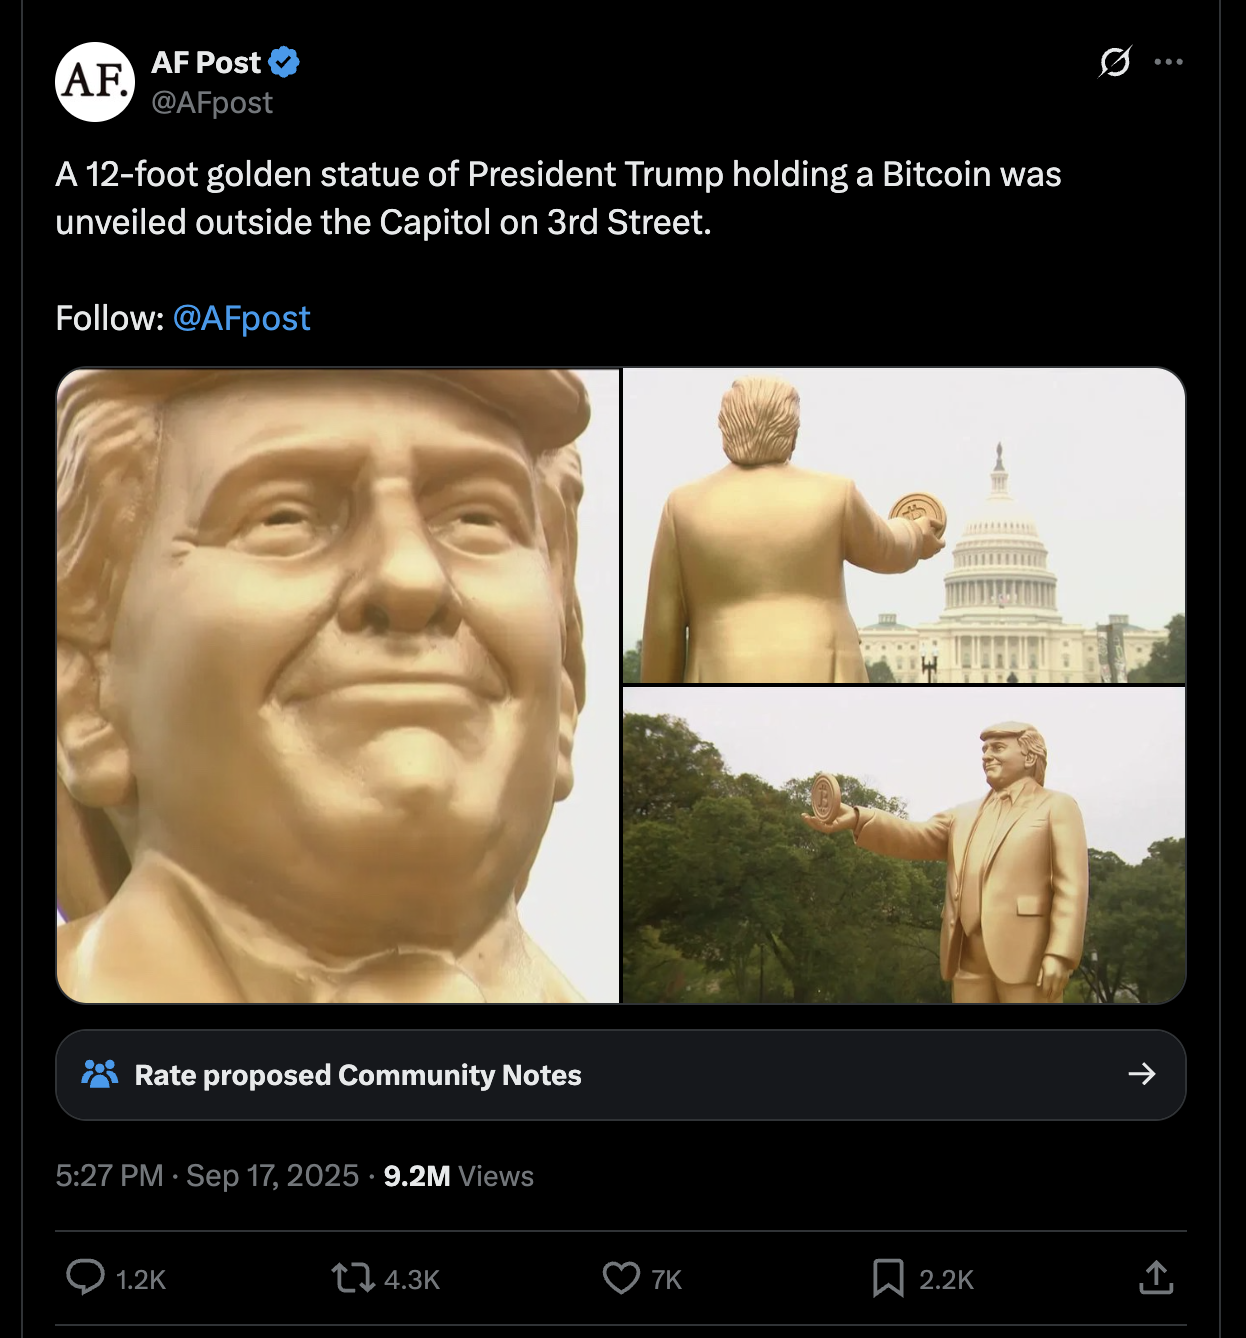
\includegraphics[height = .8\textheight]{trump.png}
\end{center}
    
\end{frame}


\begin{frame}
\frametitle{Roadmap}
\tableofcontents
\end{frame}

%------------------------------------------------

%------------------------------------------------
% insert table of content before each section or subsection
%------------------------------------------------
\AtBeginSection[]
%\AtBeginSubsection[]
{
\begin{frame}
\frametitle{Roadmap}
\tableofcontents[currentsection,currentsubsection]
%\tableofcontents[currentsection]
\end{frame}
}
%------------------------------------------------



%---------------------------------------------------------------------
%---------------------------------------------------------------------
\section{Intro}


\begin{frame}
\frametitle{Outline}

\bi
\m Brief History
\m Structure of Ethereum
\bi
\m Smart contracts
\m Gas
\m User interface
\m Data
\ei
\m L1's and L2's
\m The Market For Promises
\ei
\end{frame}

\section{History}

\begin{frame}
\frametitle{Vitalik Buterin}

\bi
\m Born in Kolomna, Russia, 1994, father a computer scientist
\m Moved to Canada at 6
\m Attended University of Waterloo, RA'd for cryptographer Ian Goldberg
\m Wrote \href{https://ethereum.org/en/whitepaper/}{Ethereum whitepaper} in 2014
\m Got \$100k Thiel fellowship in 2014, dropped out to work on Ethereum full-time
\ei

\end{frame}

\begin{frame}
\frametitle{Vitalik Buterin}

\begin{center}
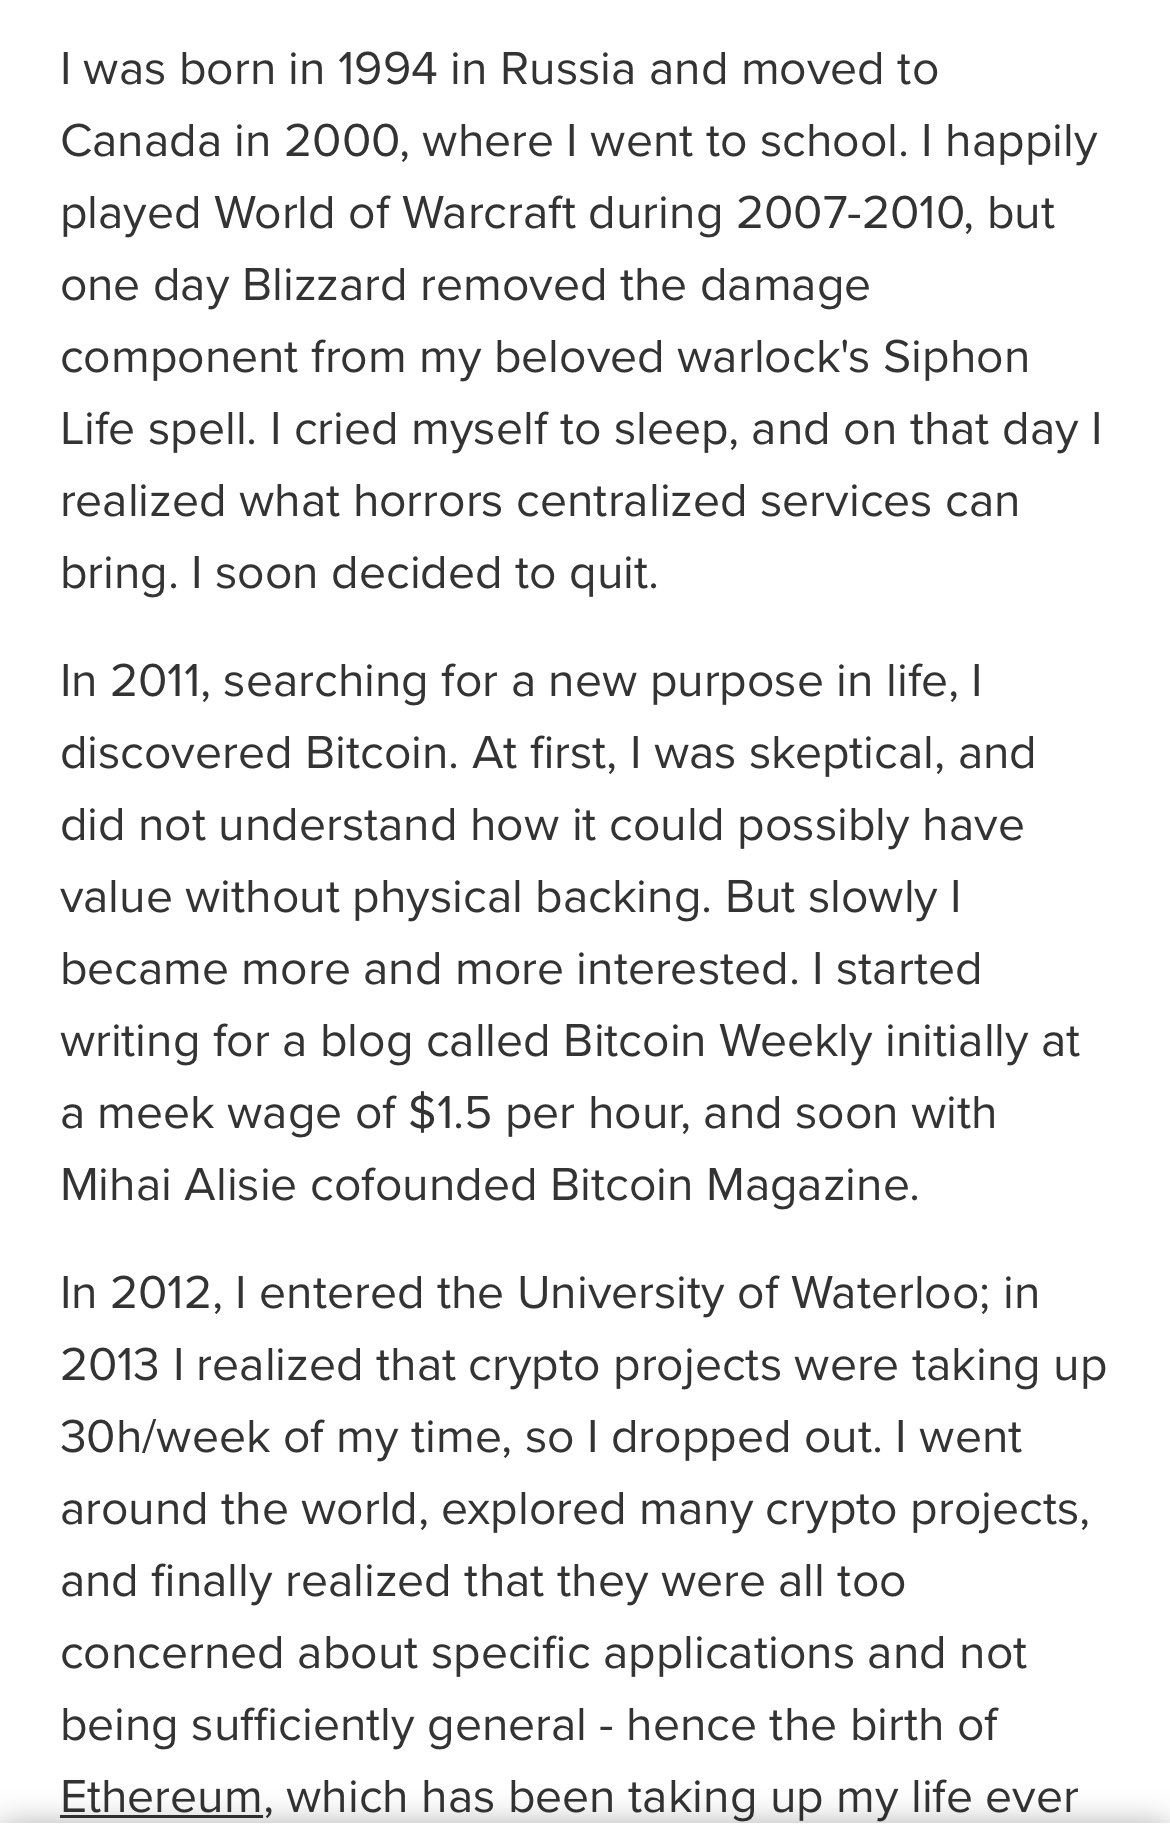
\includegraphics[width = 0.4\textwidth]{pics/wow.jpg}
\end{center}

\end{frame}

\begin{frame}
\frametitle{Application-Specific Computers}

\begin{center}
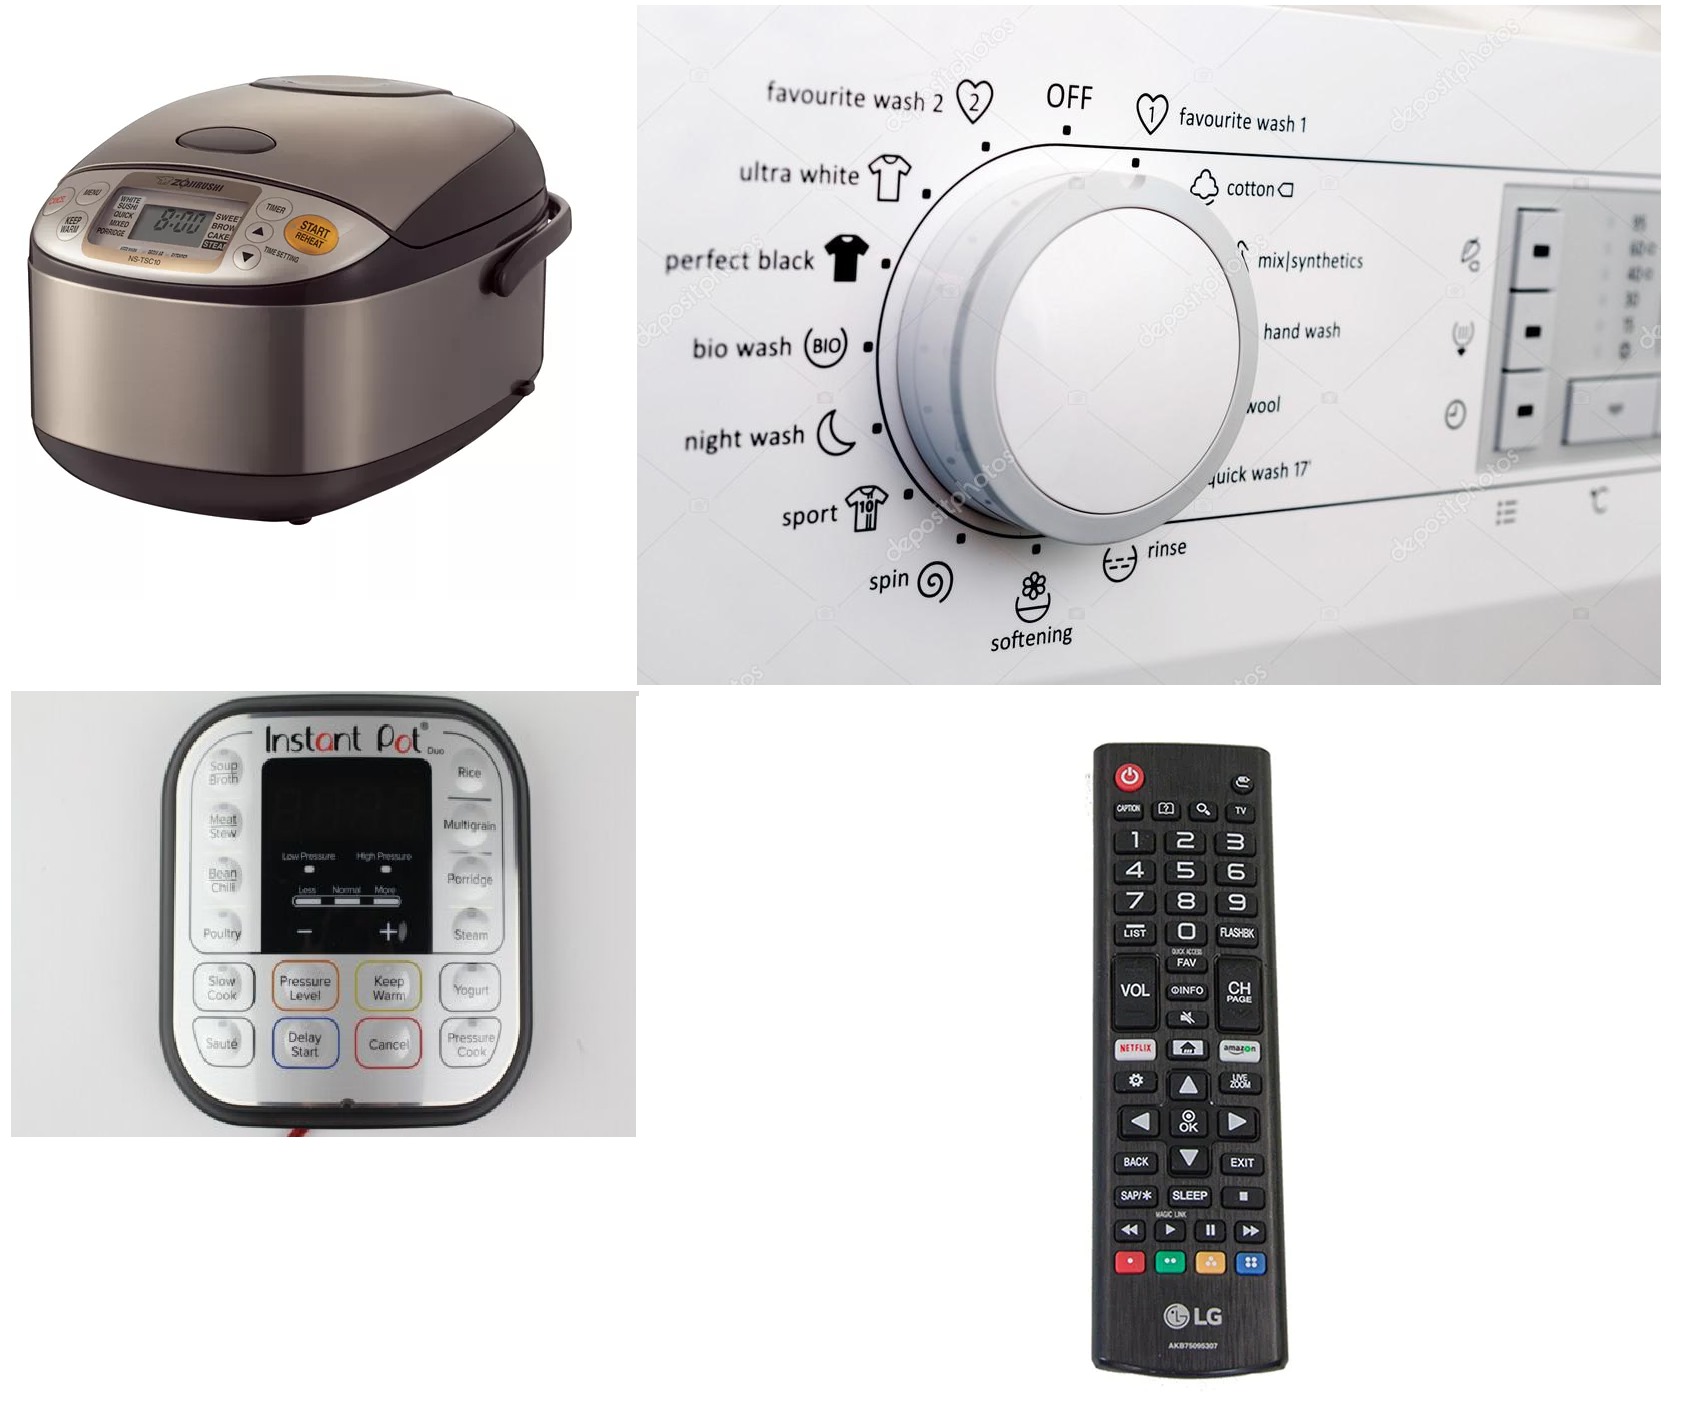
\includegraphics[width = 0.9\textwidth]{pics/appspecificcomputers.png}
\end{center}

\end{frame}


\begin{frame}
\frametitle{Universal Computers}

\bi
\m Any computing system with, essentially, if statements and ability to read data, is \ul{Turing complete}
\m Any Turing-complete language can perform same tasks as any other! \pause
\m Vitalik's insight: instead of application-specific blockchains, we should build a blockchain \ul{universal computer}
\m No need to build lots of ``buttons'': give devs a Turing-complete system, they can build their own buttons! \pause
\m Next, let's talk about the \ul{structure of Ethereum}, and how it enables universal computation
\ei

\end{frame}

\section{Structure}

\begin{frame}
\frametitle{Why learn technical details as a business major?}

``If I'm not a developer, why should I worry about the technical details?'' \pause
\bi
\m If you ``screen'' opportunities/investments: lots of BS in the space! 
\bi
\m Simple understanding of the tech helps you evaluate ideas that are ``fits'', vs pure marketing
\ei \pause
\m If you want to start a company, need to have at least a nontechnical understanding
\bi
\m What is special about the technology? What can I do that I couldn't do before?
\ei \pause
\m Hopefully, as you'll see, the tech is not \emph{that} hard
\ei

\end{frame}

\begin{frame}
\frametitle{The Structure of Ethereum}

\bi
\m Smart Contracts
\m Gas
\m User Interface
\m Data
\m Proof of Stake
\ei

\end{frame}


\subsection{Smart Contracts}

\begin{frame}{Smart Contracts}

    ``A smart contract is essentially an automated agent that lives on the Ethereum network, has an Ethereum address and balance, and can send and receive transactions. A contract is "activated" every time someone sends a transaction to it, at which point it runs its code, perhaps modifying its internal state or even sending some transactions, and then shuts down.'' \\
 
-Ethereum Whitepaper, Vitalik Buterin (2014)
    
\end{frame}


\begin{frame}
\frametitle{Smart Contracts}

\bi
\m A smart contract is:
\bi
\m A \ul{wallet}, which can hold \ul{Ether (ETH)},
\m Functions it can call when requested as determined by its \ul{code},
\m (optionally) a source of \ul{data} to which it can read and write \pause 
\ei
\m If you've heard of \ul{object oriented programming}: smart contracts are a bundle of functions (code), data, as well as ETH balances \pause
\m The most popular coding language which compiles Ethereum script code (a minimal Turing-complete language akin to assembly) is called \textbf{Solidity} \pause 
\ei
Deploying a smart contract or calling its functions requires a \textbf{gas fee}: ETH must be paid to the network to run the code. 

\end{frame}

\begin{frame}
\frametitle{Smart Contract Example: Tokens}

\bi
\m An ETH address, ``technically'', only ``holds'' Ether (``ETH'') natively -- no other tokens!
\m An ETH address can be assigned non-ETH tokens through \ul{smart contracts}
\m A \ul{smart contract} can define \ul{tokens} using the \textbf{ERC-20} standard 
\bi 
\m So-called because it was originally the 20th submission to ``Ethereum Requests for Comments'' 
\ei 
\ei

\end{frame}

\begin{frame}{Is ETH intended to store value?}

Unlike BTC, its scarcity is not strict. This is reflected in prices: 

\begin{center}
    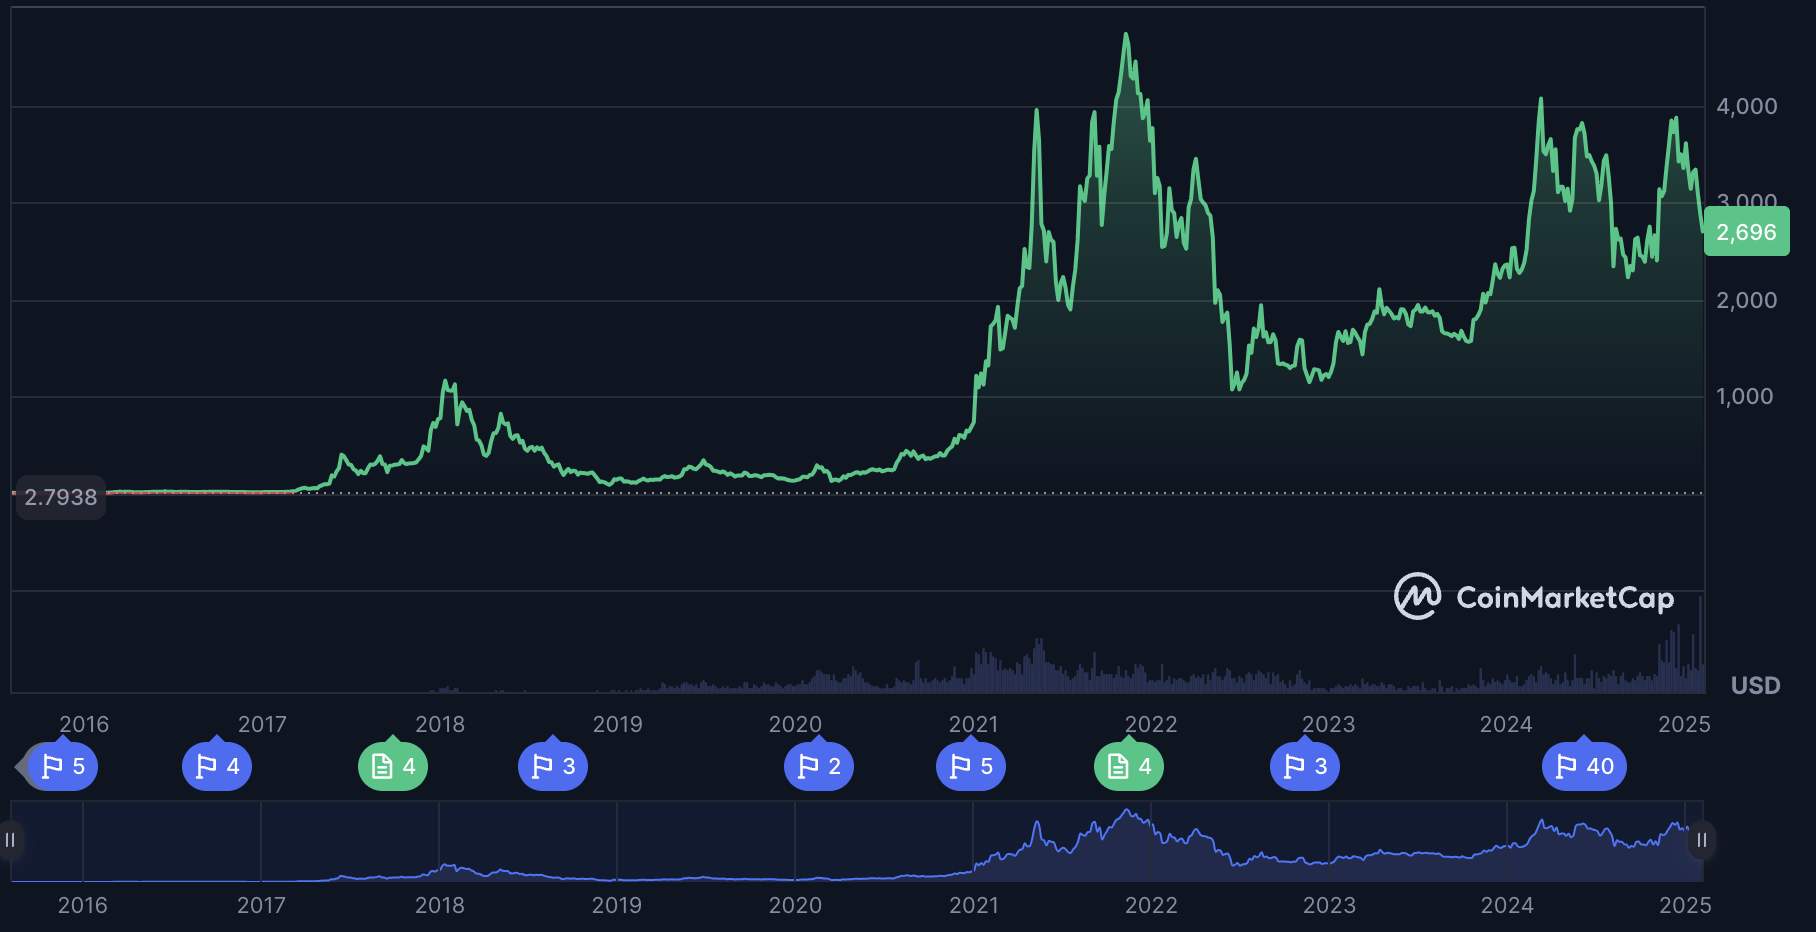
\includegraphics[width = .9\textwidth]{Screenshot 2025-02-07 at 1.20.16 PM.png}
\end{center} \pause 

\begin{itemize}
    \item This is by design: ETH itself is a currency to pay gas fees to run smart contracts \pause
    \item Think of ETH like PACE credits at GATech: kept in short supply only to ensure people don't abuse computing resources 
\end{itemize}
    
\end{frame}

\begin{frame}{The ERC-20 Standard}

The real power of the Ethereum network is the ability to create and issue new tokens with arbitrary programmable properties using \textbf{The ERC-20 Standard} \pause \vfill  

Smart contracts which issue tokens must adhere to this standard to be \ul{interoperable} with dapps (decentralized apps) \vfill \pause 
The ERC-20 Standard requires that a smart contract issuing tokens have certain functions including: 
\bi
\m Report the \ul{name} and \ul{symbol} of the token \pause 
\m \ul{Transfer} tokens from one wallet to another \pause 
\m Report the \ul{balance} of a wallet \pause 
\m Report the \ul{total supply} of the token 
\ei 
The full standard from \hyperlink{https://eips.ethereum.org/EIPS/eip-20}{eips.ethereum.org}
    
\end{frame}


\begin{frame}
\frametitle{A Token Contract in Solidity}

\begin{center}
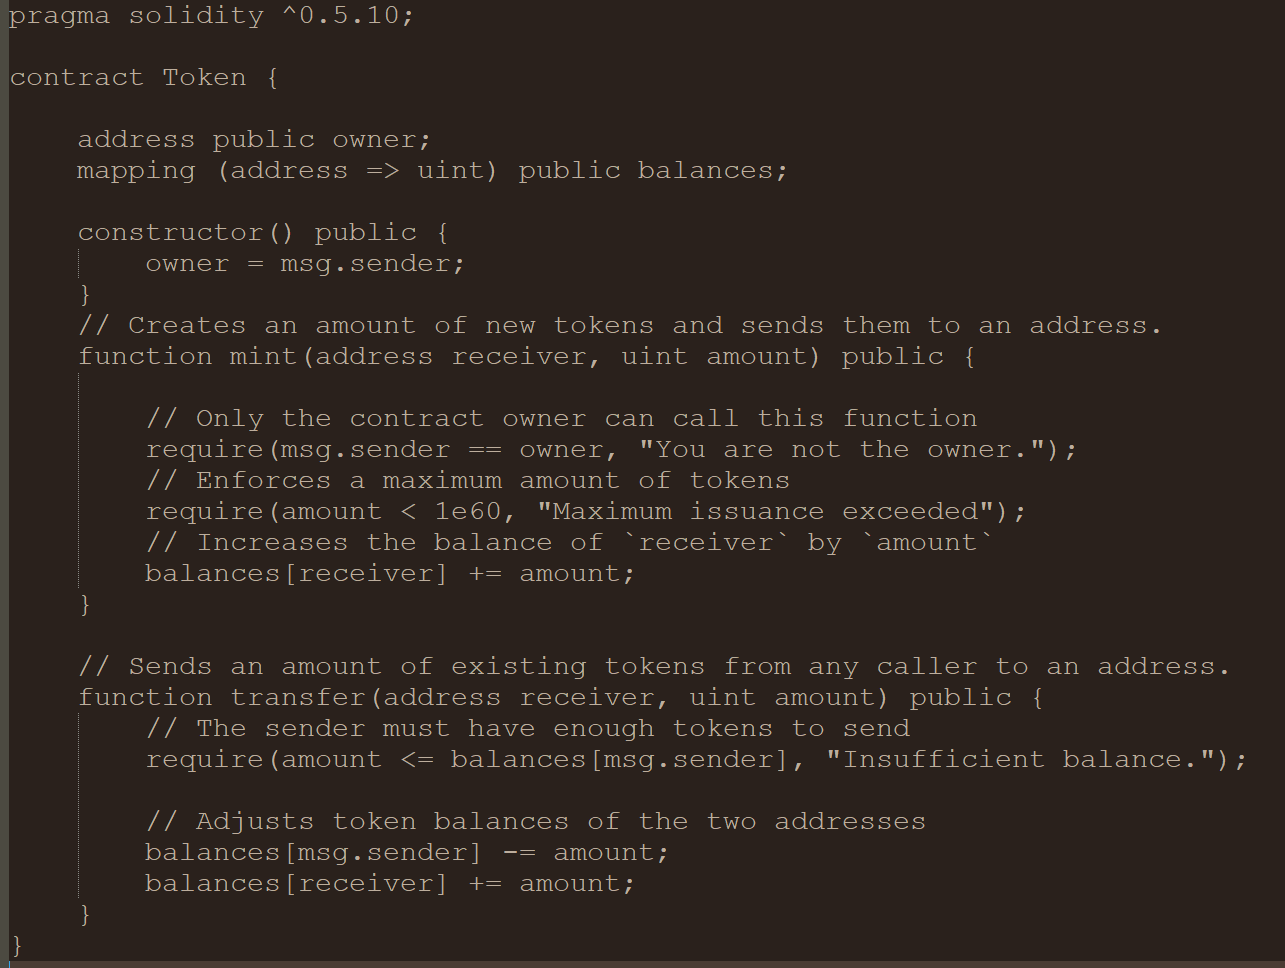
\includegraphics[width = 0.9\textwidth]{pics/tokencontractcode.png}
\end{center}

\footnotesize
Source: \href{https://ethereum.org/en/developers/docs/smart-contracts/anatomy/}{ETH documentation}

\end{frame}

\begin{frame}
\frametitle{Can Smart Contracts be Changed?}

\pause
\bi
\m \ul{Code} cannot change, but \ul{data} can 
\m Trick: use data to reference code! 
\m Make a ``proxy contract'' A, which has ``implementation'' address X, and simply calls the contract at X
\m If you change X, you change what A does!
\ei

Source: \href{https://ethereum.org/en/developers/docs/smart-contracts/upgrading/}{ETH documentation}

\end{frame}

\begin{frame}
\frametitle{Can Smart Contracts be Changed?}

Picture: forwarding addresses

\end{frame}

\begin{frame}
\frametitle{Can Smart Contracts be Changed?}

Potentially important for: 
\bi
\m Security: can devs change code and steal my money? \pause
\m Legal implications: can devs conceivably change code, hence are they responsible for behavior of code? 
\ei

\end{frame}


\begin{frame}
\frametitle{Can Smart Contracts be Changed?}

Takeaways: 
\bi
\m Smart contracts can be built in a way that makes them upgradable
\m But (from the code) you can tell whether a smart contract is upgradable or not
\m Devs can \ul{commit} to never update a piece of code by hard-coding functions into the \ul{public} solidity code \pause 
\m \textbf{or}, Devs can avoid committing to that promise by writing functions that reference other sources of data (which can in principle be indecipherable to the public) 
\m Thus, developers face a \textbf{tradeoff}: contracts may be either \emph{upgradeable and private} \underline{or} \emph{public and immutable} -- they can never be both. 
\ei

\end{frame}

\begin{frame}
\frametitle{Can you tell what the code in a smart contract is?}

\pause
\bi
\m Smart contracts on ETH store a \ul{code hash} of compiled EVM code
\m Given Solidity code, can check whether compiled code hashes to contract address
\m However, can't reverse the hash: can only verify correctness if code is submitted
\m Developers can voluntarily publish their code (and anyone can verify that it matches the compiled code hash)
\ei

\end{frame}

\begin{frame}
\frametitle{Can you tell what code in a smart contract is?}

\begin{center}
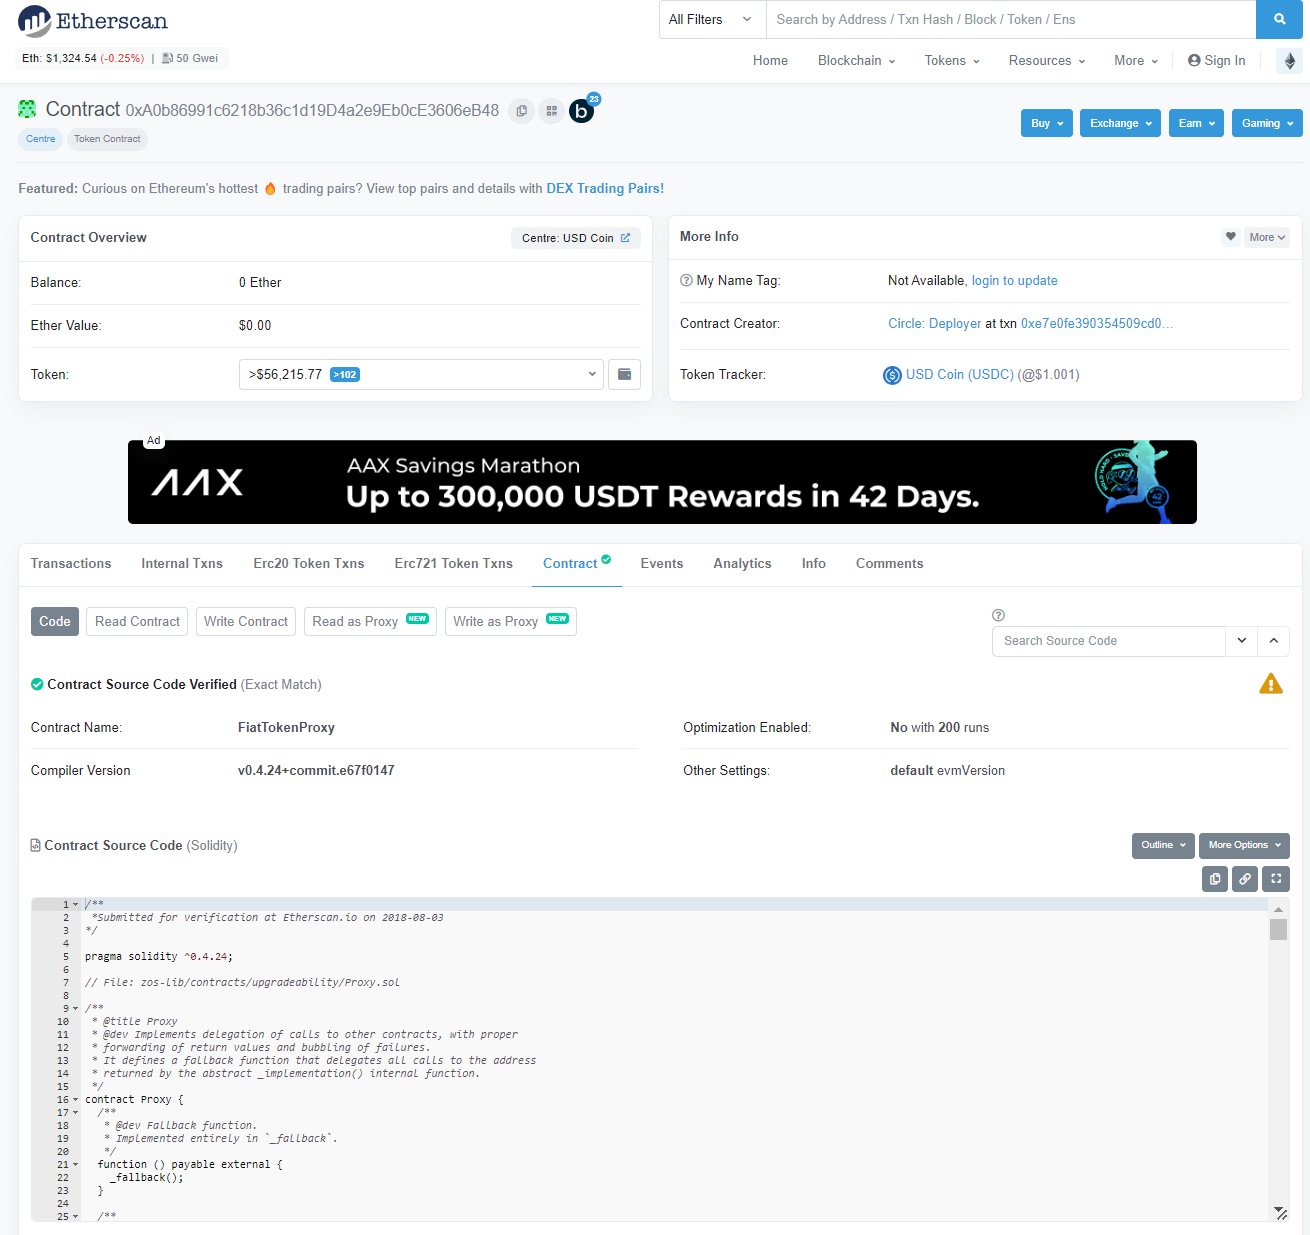
\includegraphics[width = 0.8\textwidth]{pics/usdc_contract.png}
\end{center}

\end{frame}

\begin{frame}{Uniswap is (essentially) a Smart Contract}

\begin{center}
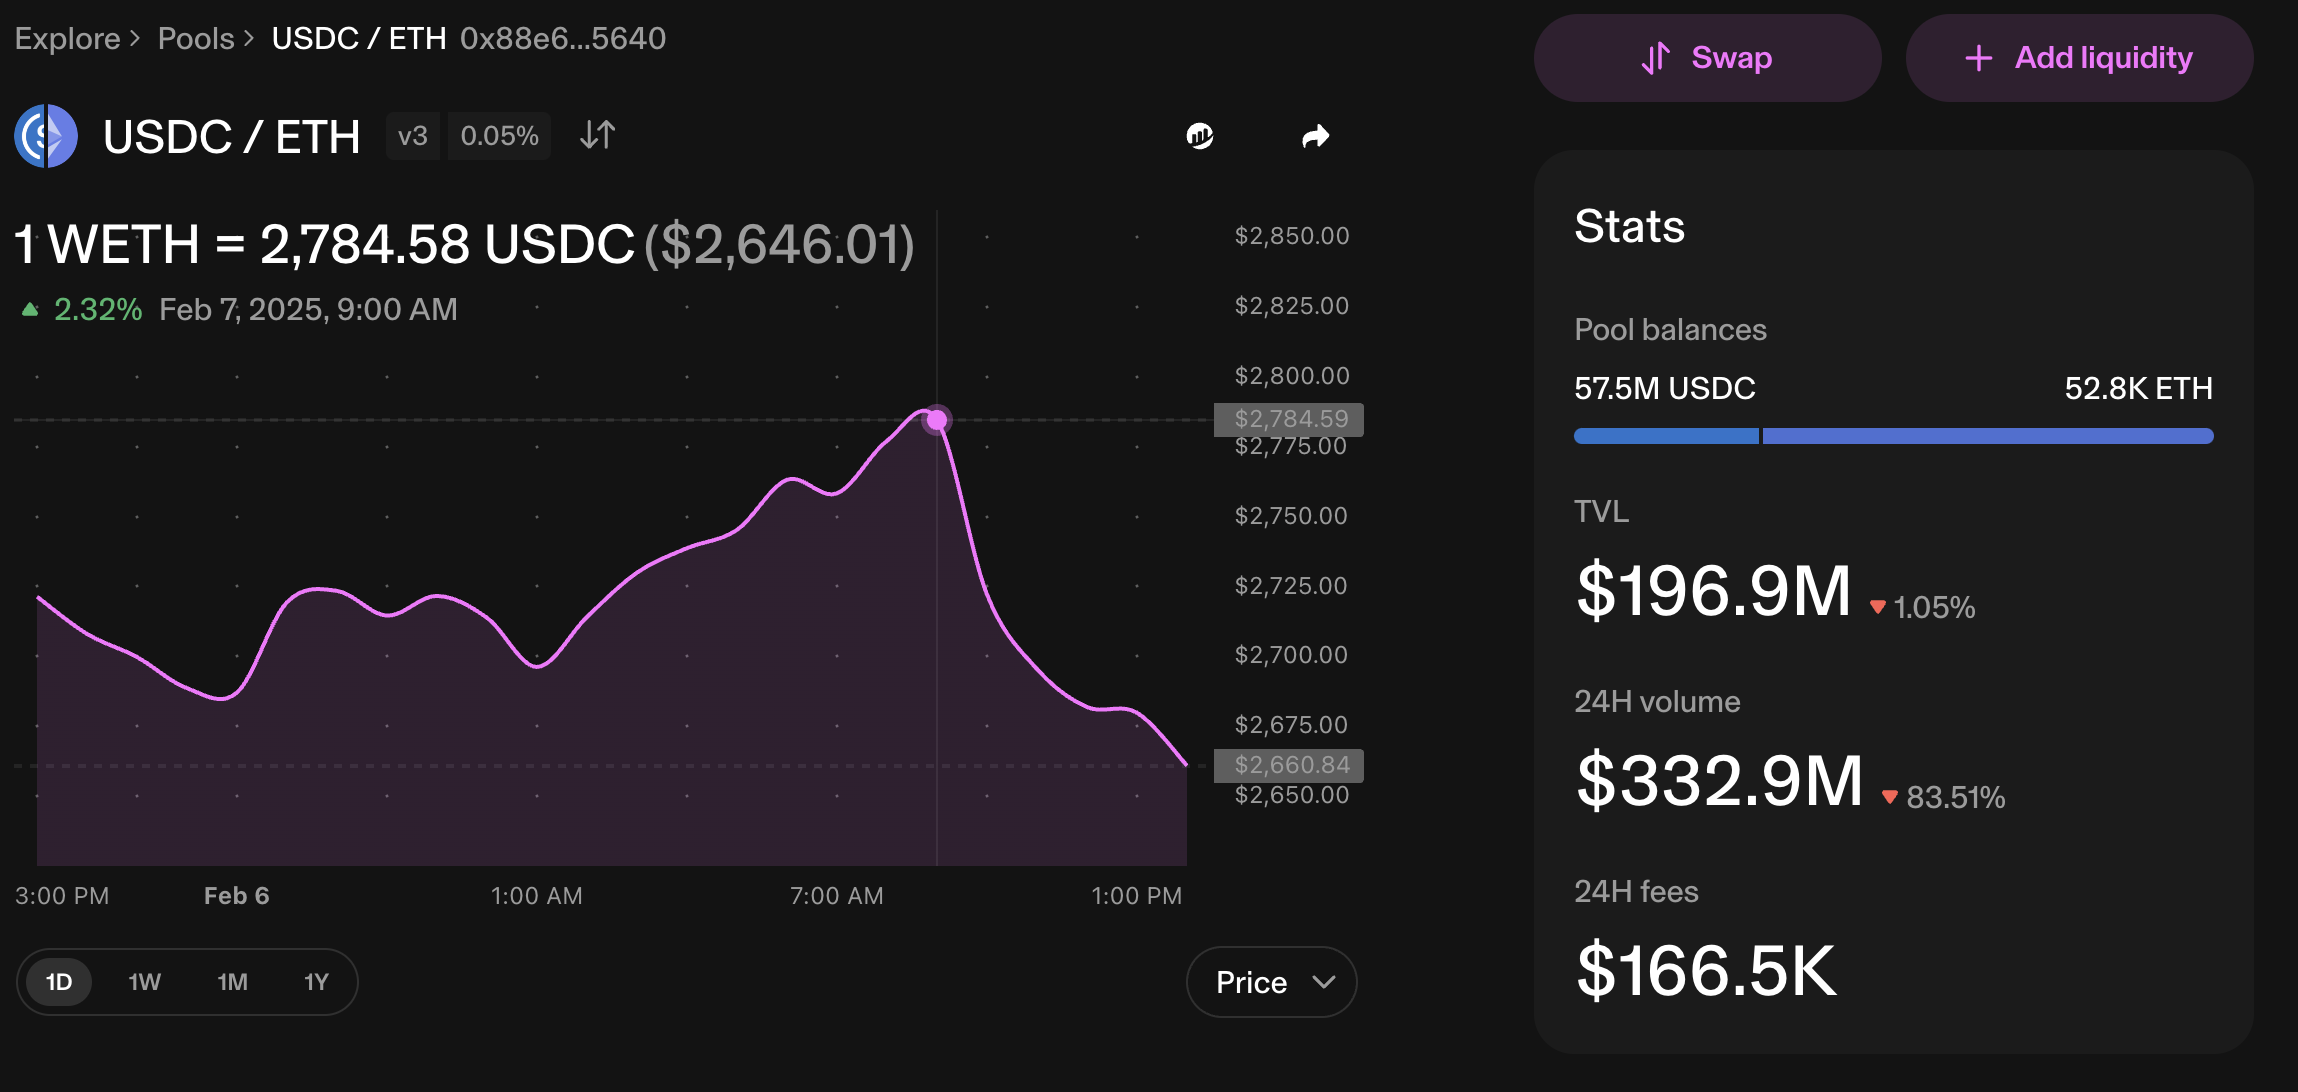
\includegraphics[width = \textwidth]{Screenshot 2025-02-07 at 3.22.43 PM.png}
\end{center}

    
\end{frame}


\begin{frame}
\frametitle{Smart Contracts and Regulation}


\begin{center}
\includegraphics<1>[width = 0.9\textwidth]{pics/tornadocash.png}
\includegraphics<2>[width = 0.9\textwidth]{pics/uniswapsuit1.png}
\includegraphics<3>[width = 0.7\textwidth]{pics/uniswapsuit2.png}
\includegraphics<4>[width = 0.7\textwidth]{pics/uniswapsuit3.png}
\end{center}

\end{frame}

\begin{frame}{Is Uniswap a Securities Exchange?}

From Uniswap's letter to the SEC: \\

\textbf{The Protocol Is an Automated Market Maker Technology Controlled by No Individual or Entity.} \\

{\tiny The Protocol is an autonomous set of ``smart contracts''
 that run on the Ethereum network—that is, software on the Ethereum blockchain programmed to automatically execute trades, akin to a pre-programmed digital vending machine. The Protocol is the first widely successful automated market maker (“AMM”), and relies on LPs contributing liquidity into a liquidity pool that generally contains two specific assets. Liquidity pools represent the quantity of assets that users in the aggregate are willing to have swapped at prices determined using a constant-product market maker formula (x*y = k), which automatically rebalances with swaps as the ratios of various assets fluctuate. The formula ensures that the product of x and y, representing the balance of the two tokens in any pool, equals a constant, k. Because the relative price of the assets can be changed only through trading, divergences between the Protocol price and external prices create market opportunities. The combination of the formula plus the rebalancing mechanism thus ensures that Protocol prices always trend toward the market clearing price. 
    }

\end{frame}


%        For Monday: Please read \href{https://www.drorpoleg.com/in-praise-of-ponzis/}{In Praise of Ponzis} by Dror Poleg 


\begin{frame}{Welcome! Today is Wednesday September 24, 2025}

\begin{center}
    No quiz today, roll call instead. \\
    Homework 3 has been published to Canvas. It is due a week from Monday (10/6) at the start of class. 
\end{center}
    
\end{frame}

\section{The Market For Promises}

\begin{frame}{Gudied Discussion: the Market for Promises}

\textbf{Q}: How would we summarize Anthony's argument? \\ \pause 

\textbf{A}: Since Smart Contracts/DeFi is naturally a \ul{substitute} for effective governments, the future of DeFi will be built in places with ineffective governments. \\ \pause 

\textbf{Q}: What are arguments for and against this  \\ \pause 

\textbf{For:} 
\begin{itemize}
    \item Dysfunctional legal systems make DeFi’s neutrality more valuable (demand side)
    \item Low state capacity = weak ability to suppress blockchain adoption (supply side) 
\end{itemize}

\\ \pause 

\textbf{Against:} 

\begin{itemize}
    \item Poor infrastructure, connectivity, and literacy hinder DeFi uptake. 
    \item Capital and liquidity still concentrate in developed markets.
\end{itemize}

\end{frame}


\begin{frame}
\frametitle{The Market For Promises}

Anthony Lee Zhang's \href{https://anthonyleezhang.substack.com/p/the-market-for-promises}{blog post}
\bi
\m Many pieces of human society are based on \ul{promises}
\bi
\m Financial assets (stocks, loans/bonds, derivatives\ldots) \pause
\m Firms (Employment, trade agreements\ldots) \pause
\m Religions, governments, communities \ldots \pause
\ei
\m Promises involve \ul{trust}! Finance, firms, and organizations only work if people keep their promises! \pause
\m Trust derives from a system for \ul{promise enforcement}: the legal system and the government's monopoly on violence \pause
\m But many people can't use these systems! \pause
\bi
\m Non-US groups in low state capacity countries \pause
\m Criminal organizations \pause
\ei
\ei

\end{frame}

\begin{frame}
\frametitle{The Market For Promises}

\begin{center}
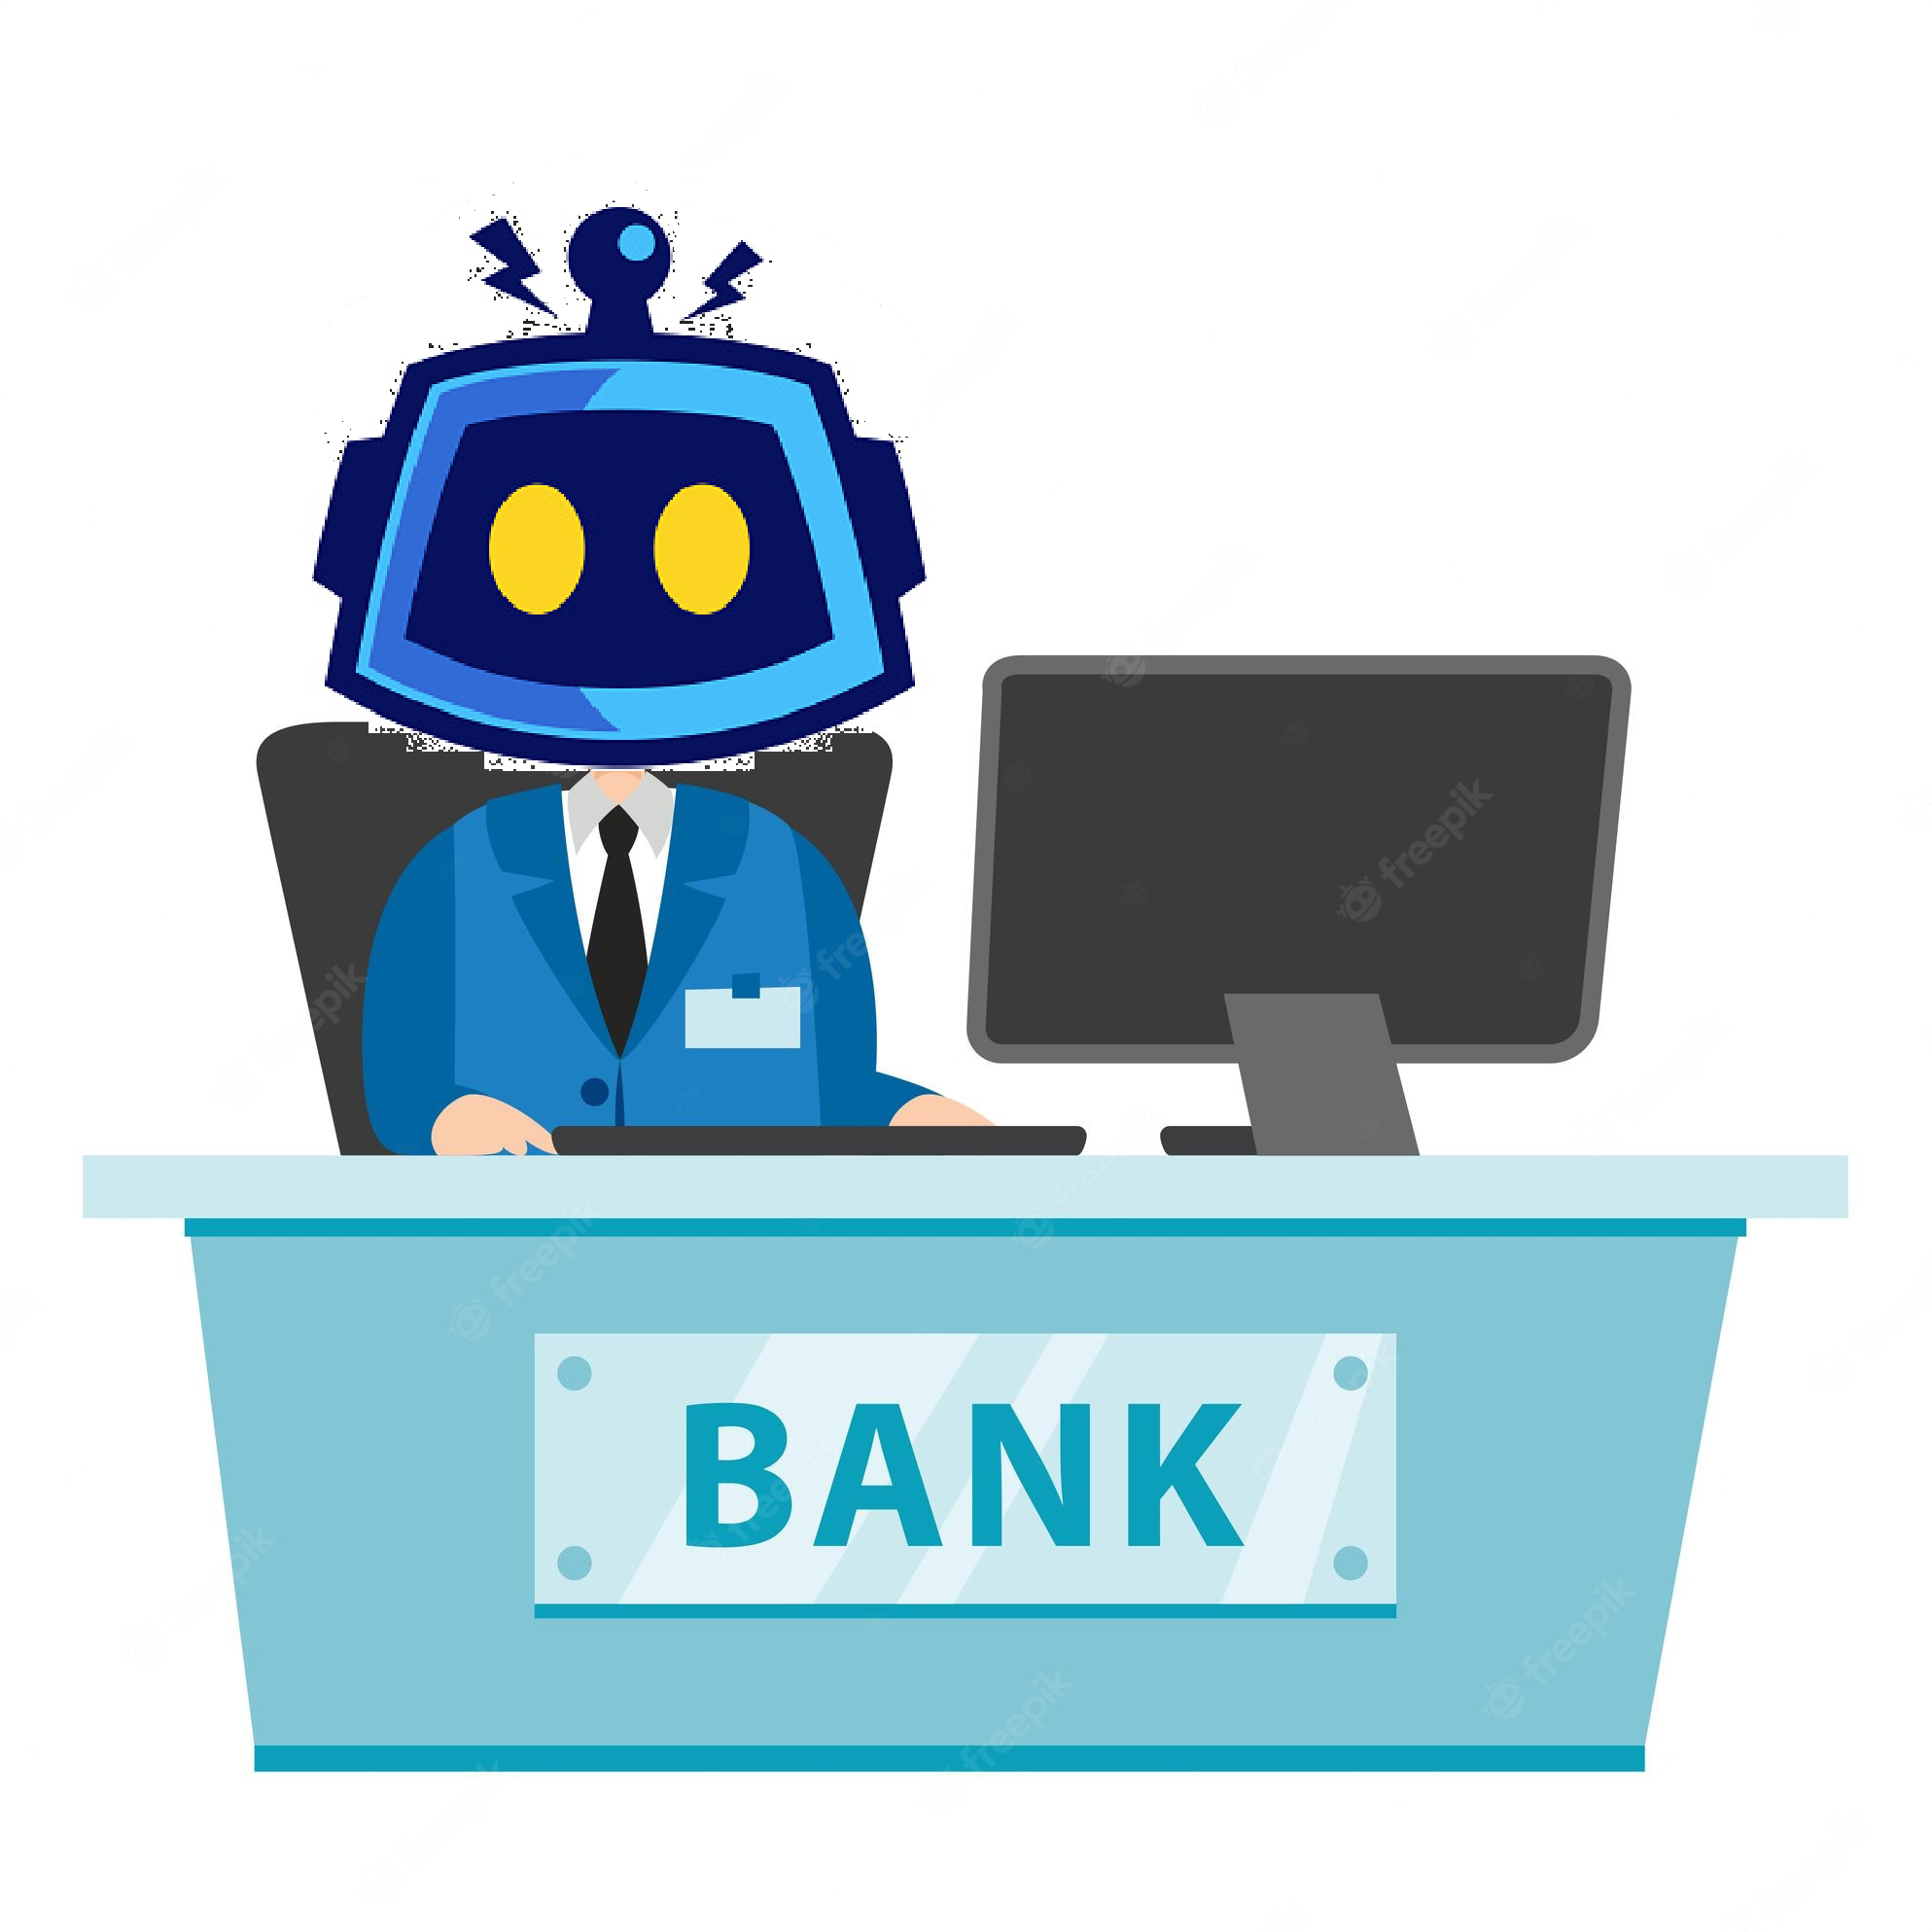
\includegraphics[width=0.2\textwidth]{pics/bankerbot.png}
\end{center}
\bi
\m BankBot (``BB'') is an \ul{alternative promise enforcement technology!}\pause
\m BB sees valid tx's submitted by Alice (sends, votes, bets\ldots) \pause
\m BB can't steal Alice's money, without Alice's private key \pause
\m BB can't change Alice's tx's, without Alice's key \pause
\m All stakers can do is ``execute'' Alice's tx's, putting them in the chain and collecting gas fees \pause
\m Stakers could try to boycott Alice's tx's\ldots \pause
\bi
\m But there's many other stakers happy to collect Alice's gas fees, and BB can't fight longest chain
\ei
\ei

\end{frame}

\begin{frame}
\frametitle{Blockchains and Access}

\begin{center}
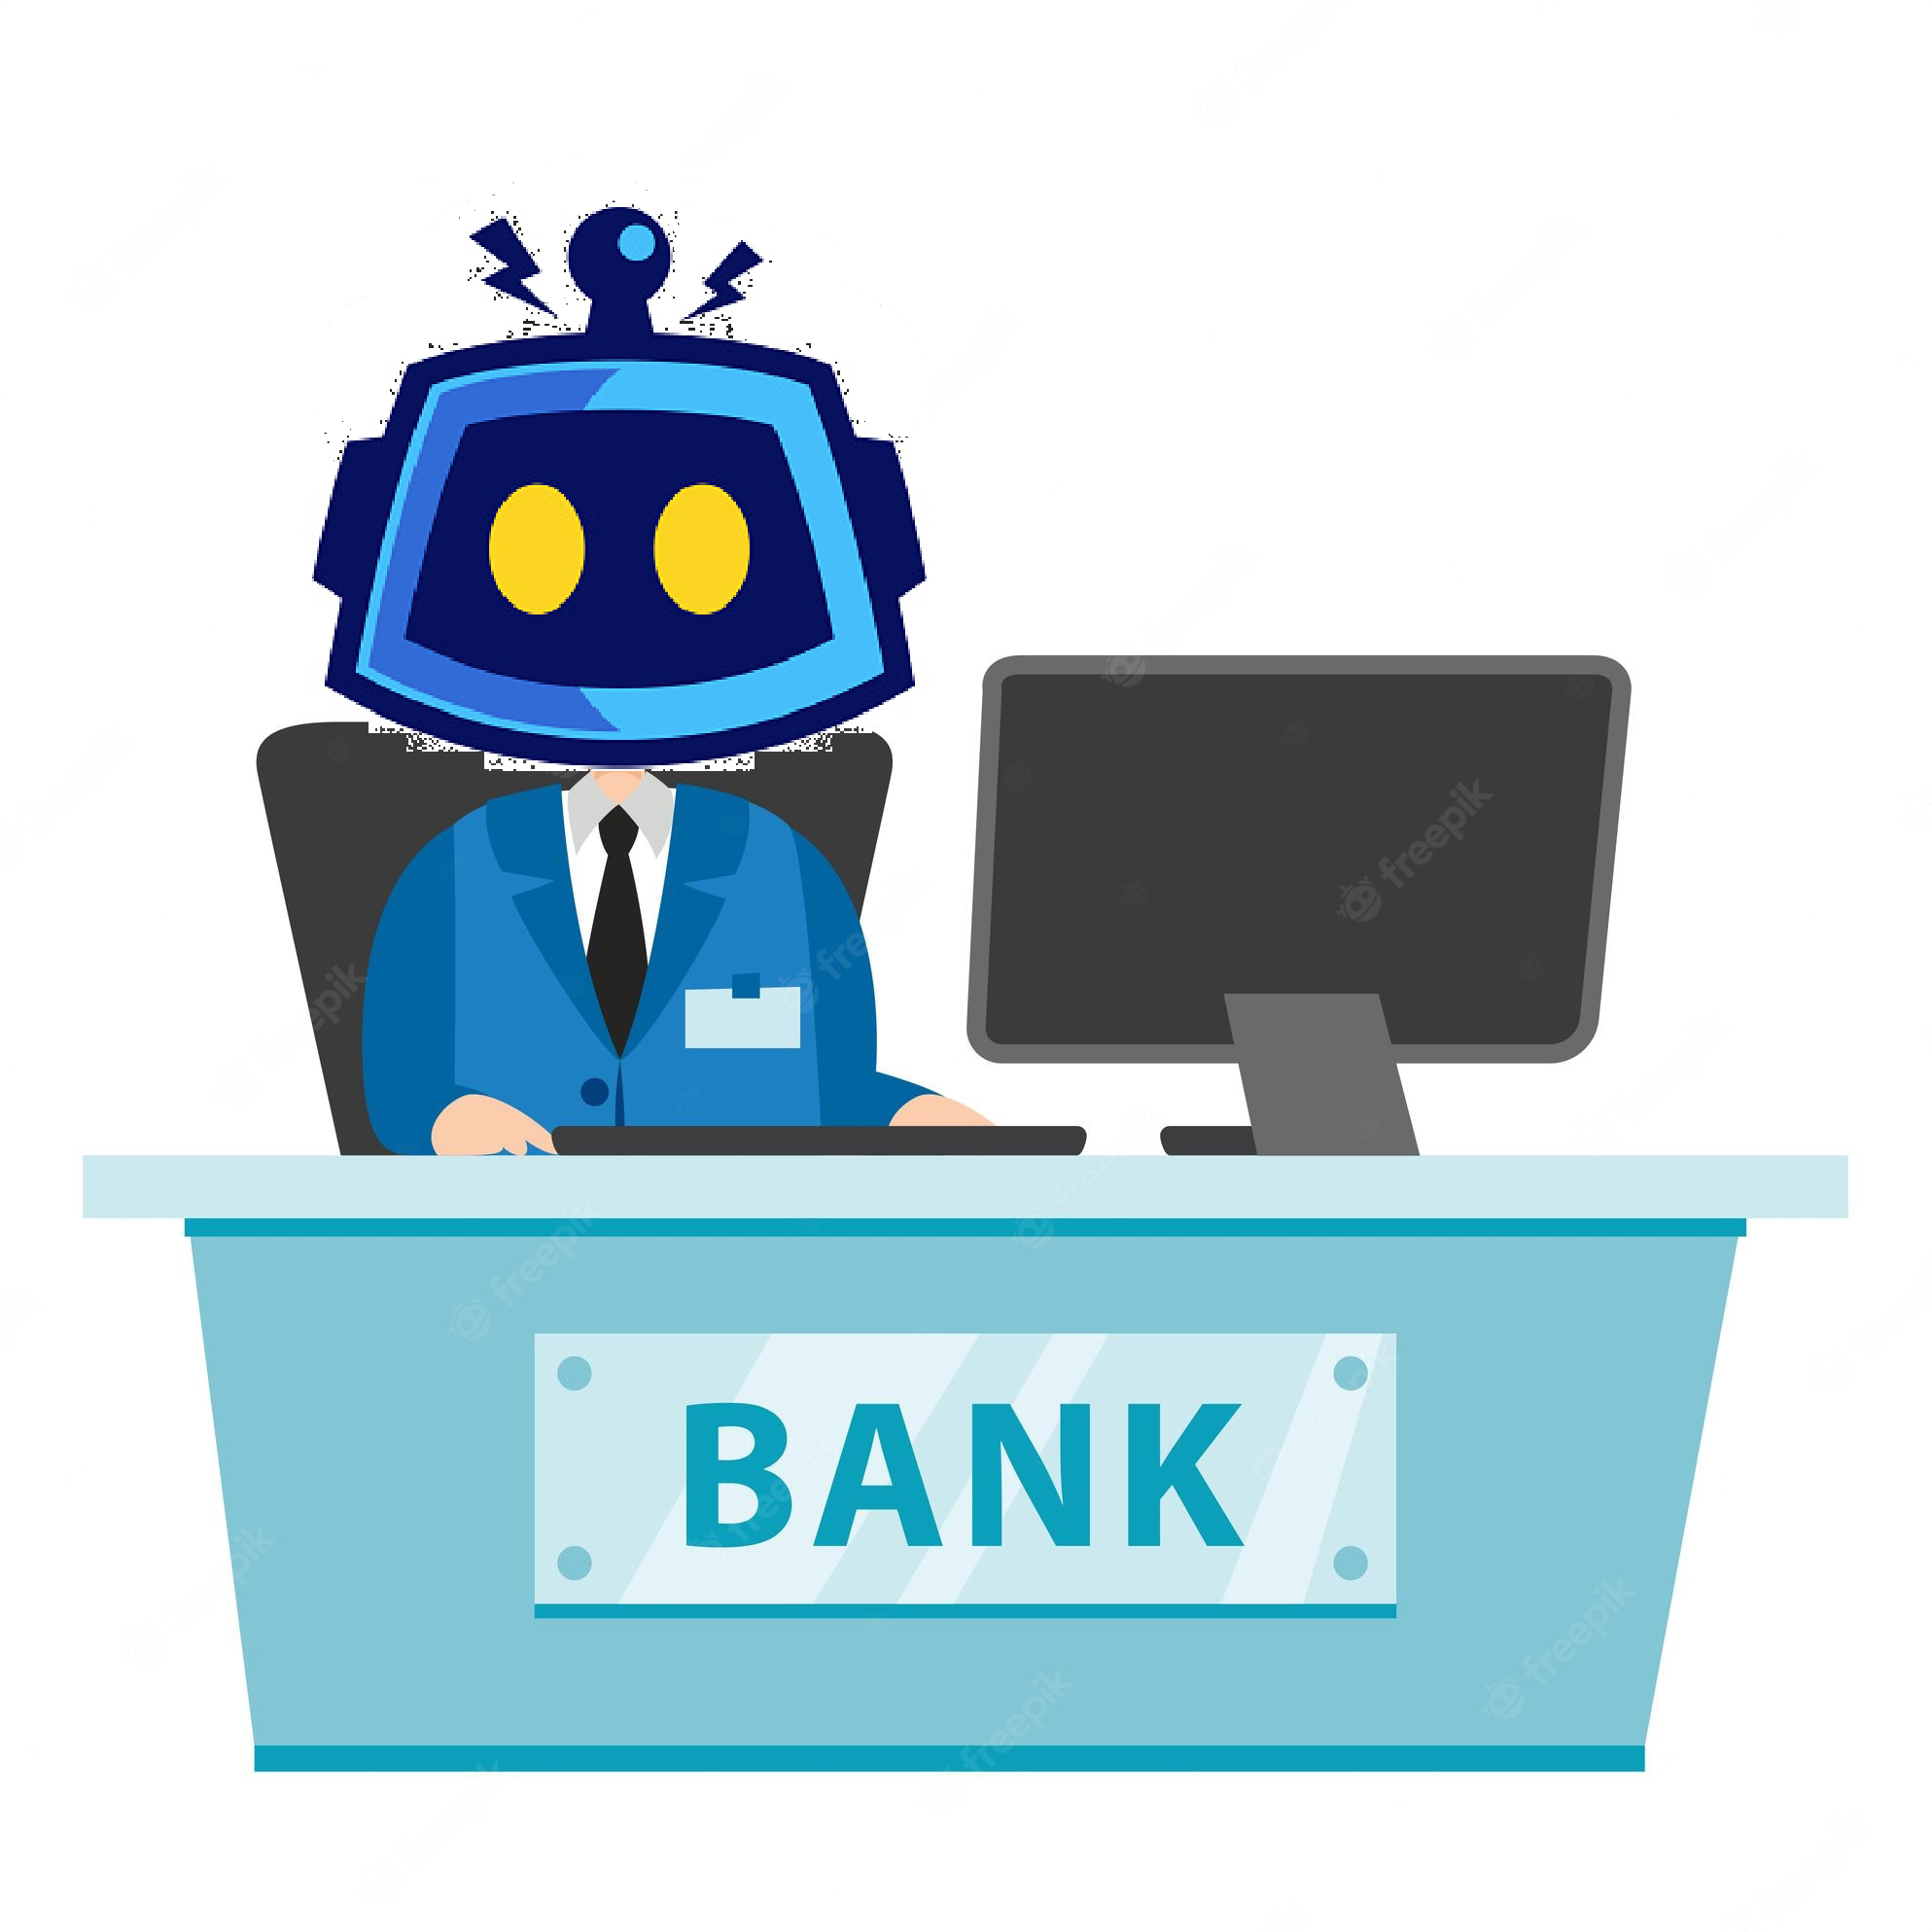
\includegraphics[width=0.2\textwidth]{pics/bankerbot.png}
\end{center}
\bi
\m Relative to court systems, blockchains are \ul{low-cost}, and have very low \ul{barriers to access}
\m Anyone with an internet connection can make promises on blockchains!
\m Costs fairly low, rel. to hiring lawyers + going to court in high-income countries
\ei

\end{frame}

\begin{frame}
\frametitle{Limits of the Market}

\begin{center}
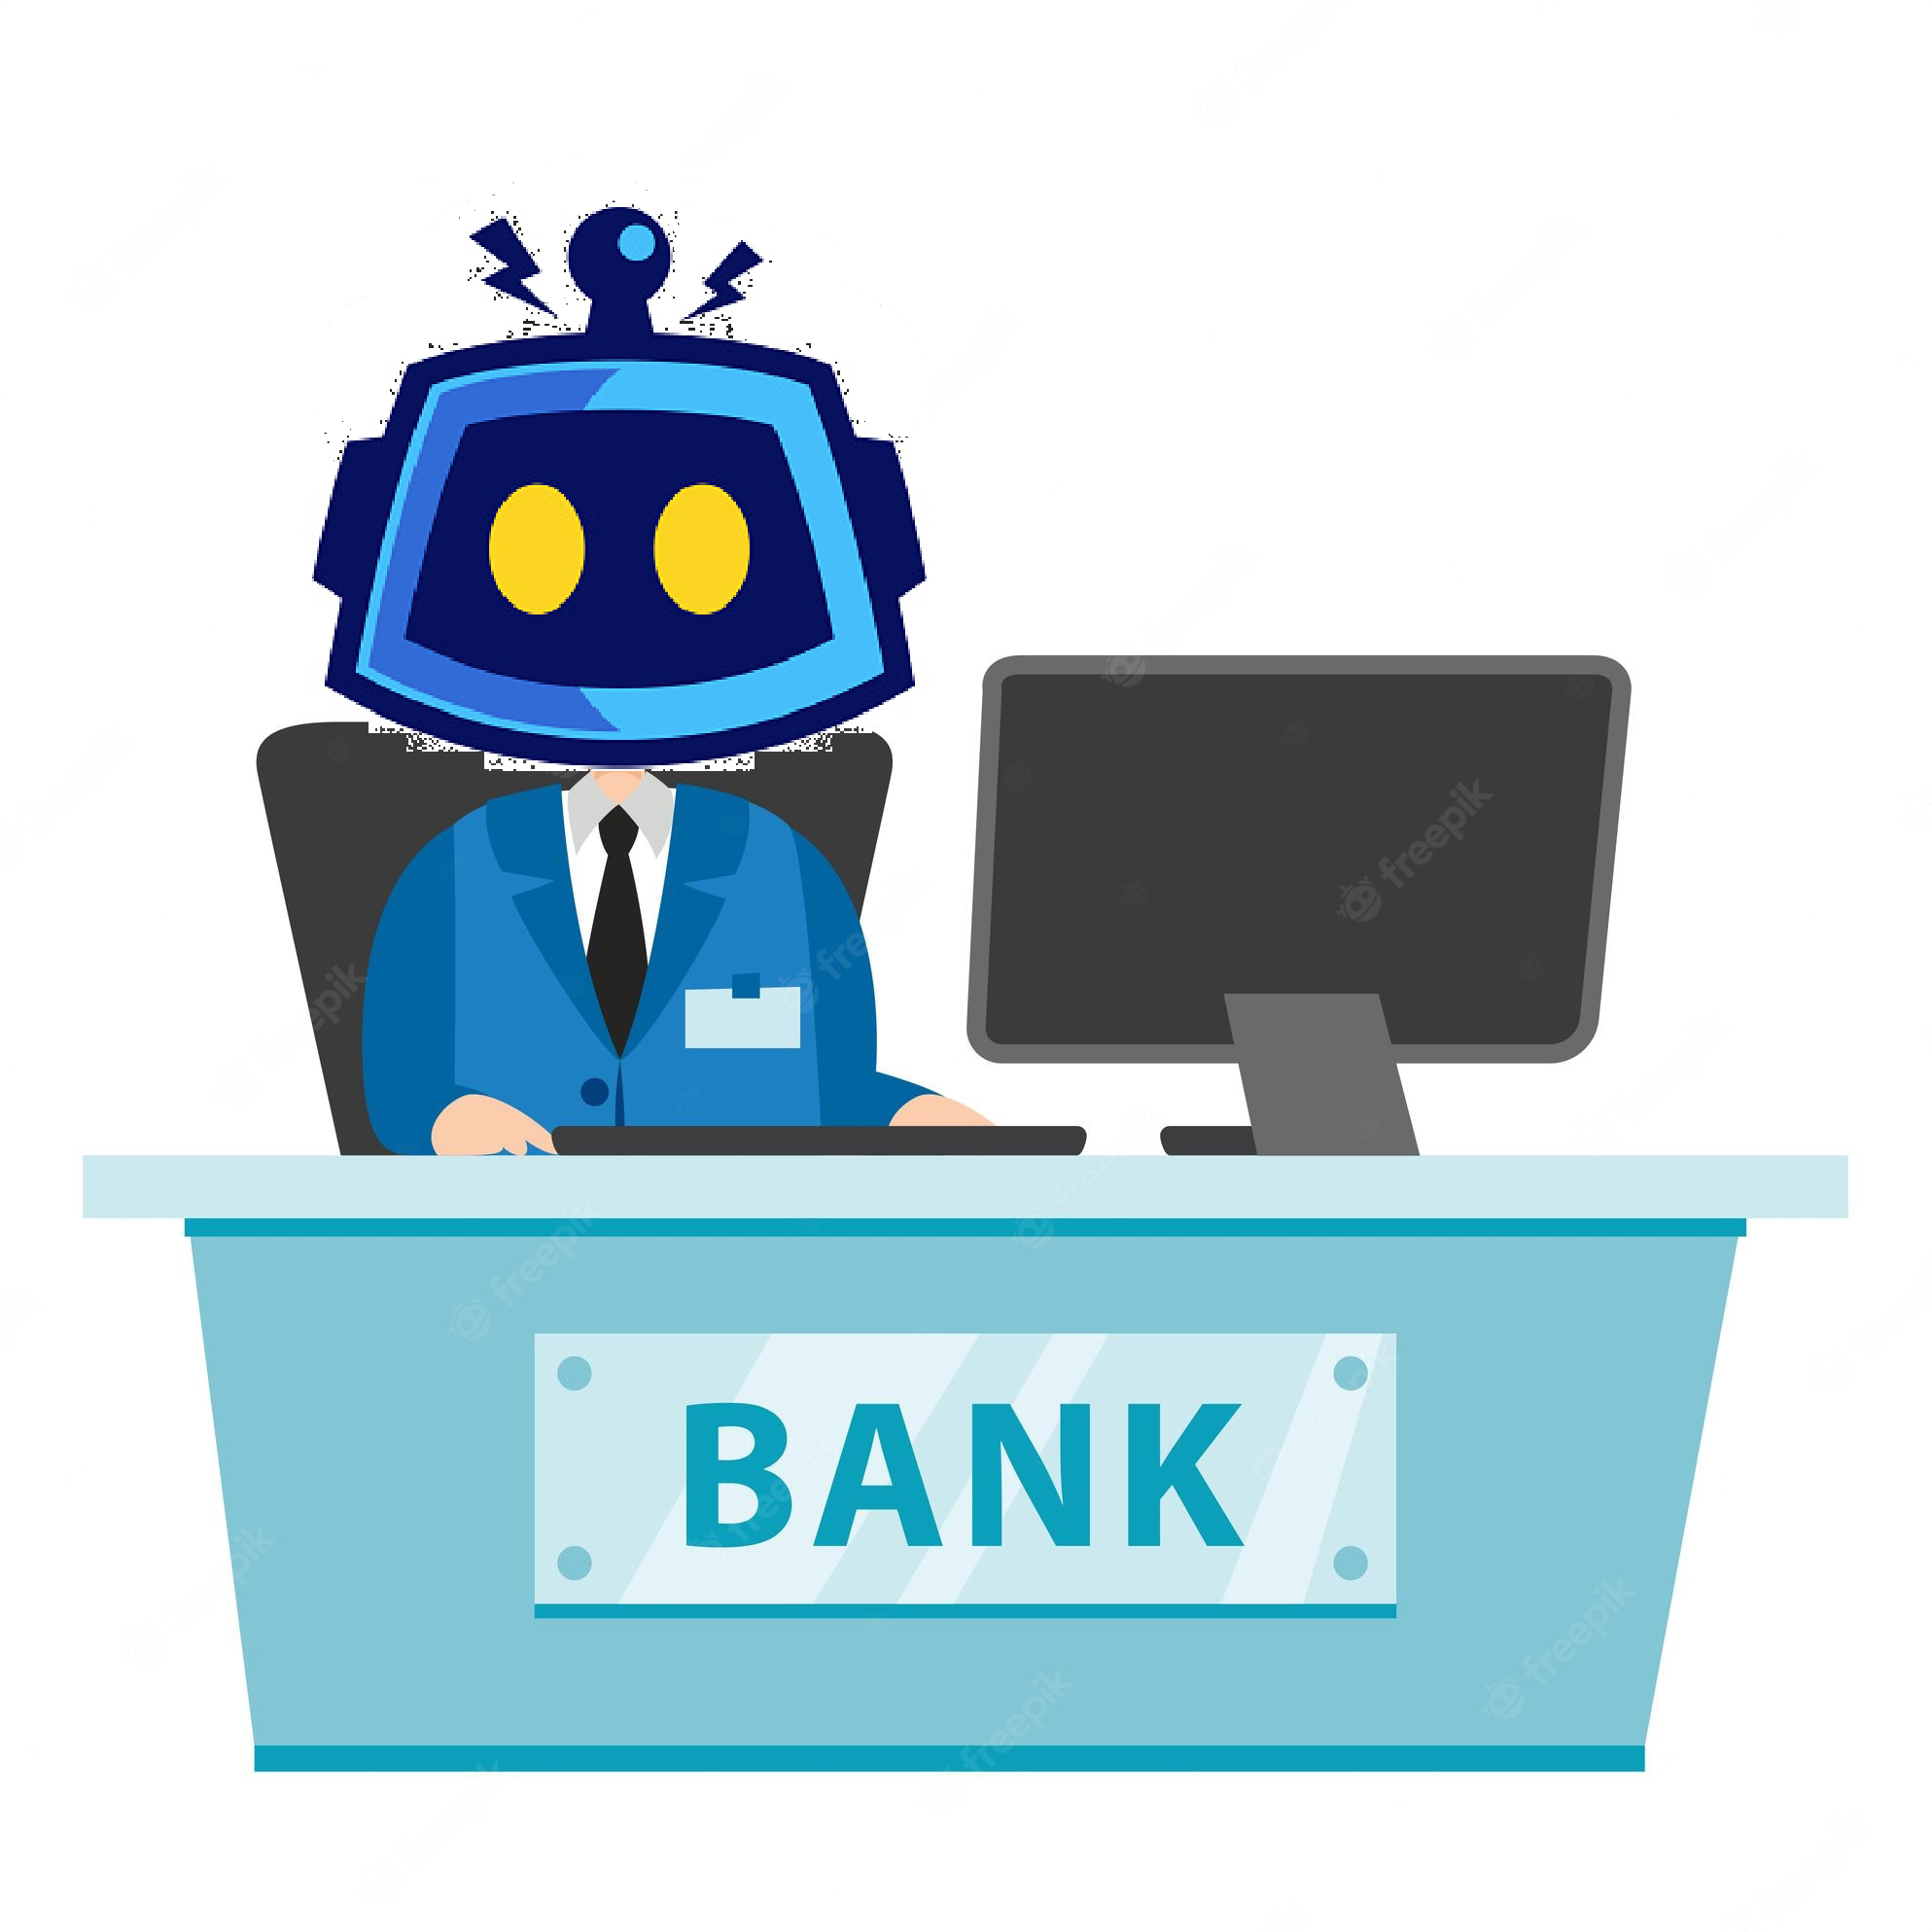
\includegraphics[width=0.2\textwidth]{pics/bankerbot.png}
\end{center}
\bi
\m Blockchains can only keep promises involving \ul{on-chain assets and events} \pause
\m If there exist valuable on-chain assets, this is a pretty big set of promises! \pause
\bi
\m Generalized financial derivatives \pause
\m Generalized voting mechanisms \pause
\ei 
\m Some core problems: \pause
\bi
\m Referencing \ul{real world assets and events} is hard 
\ei
\ei

\end{frame}

\begin{frame}
\frametitle{Blockchains and Discretion}

\begin{center}
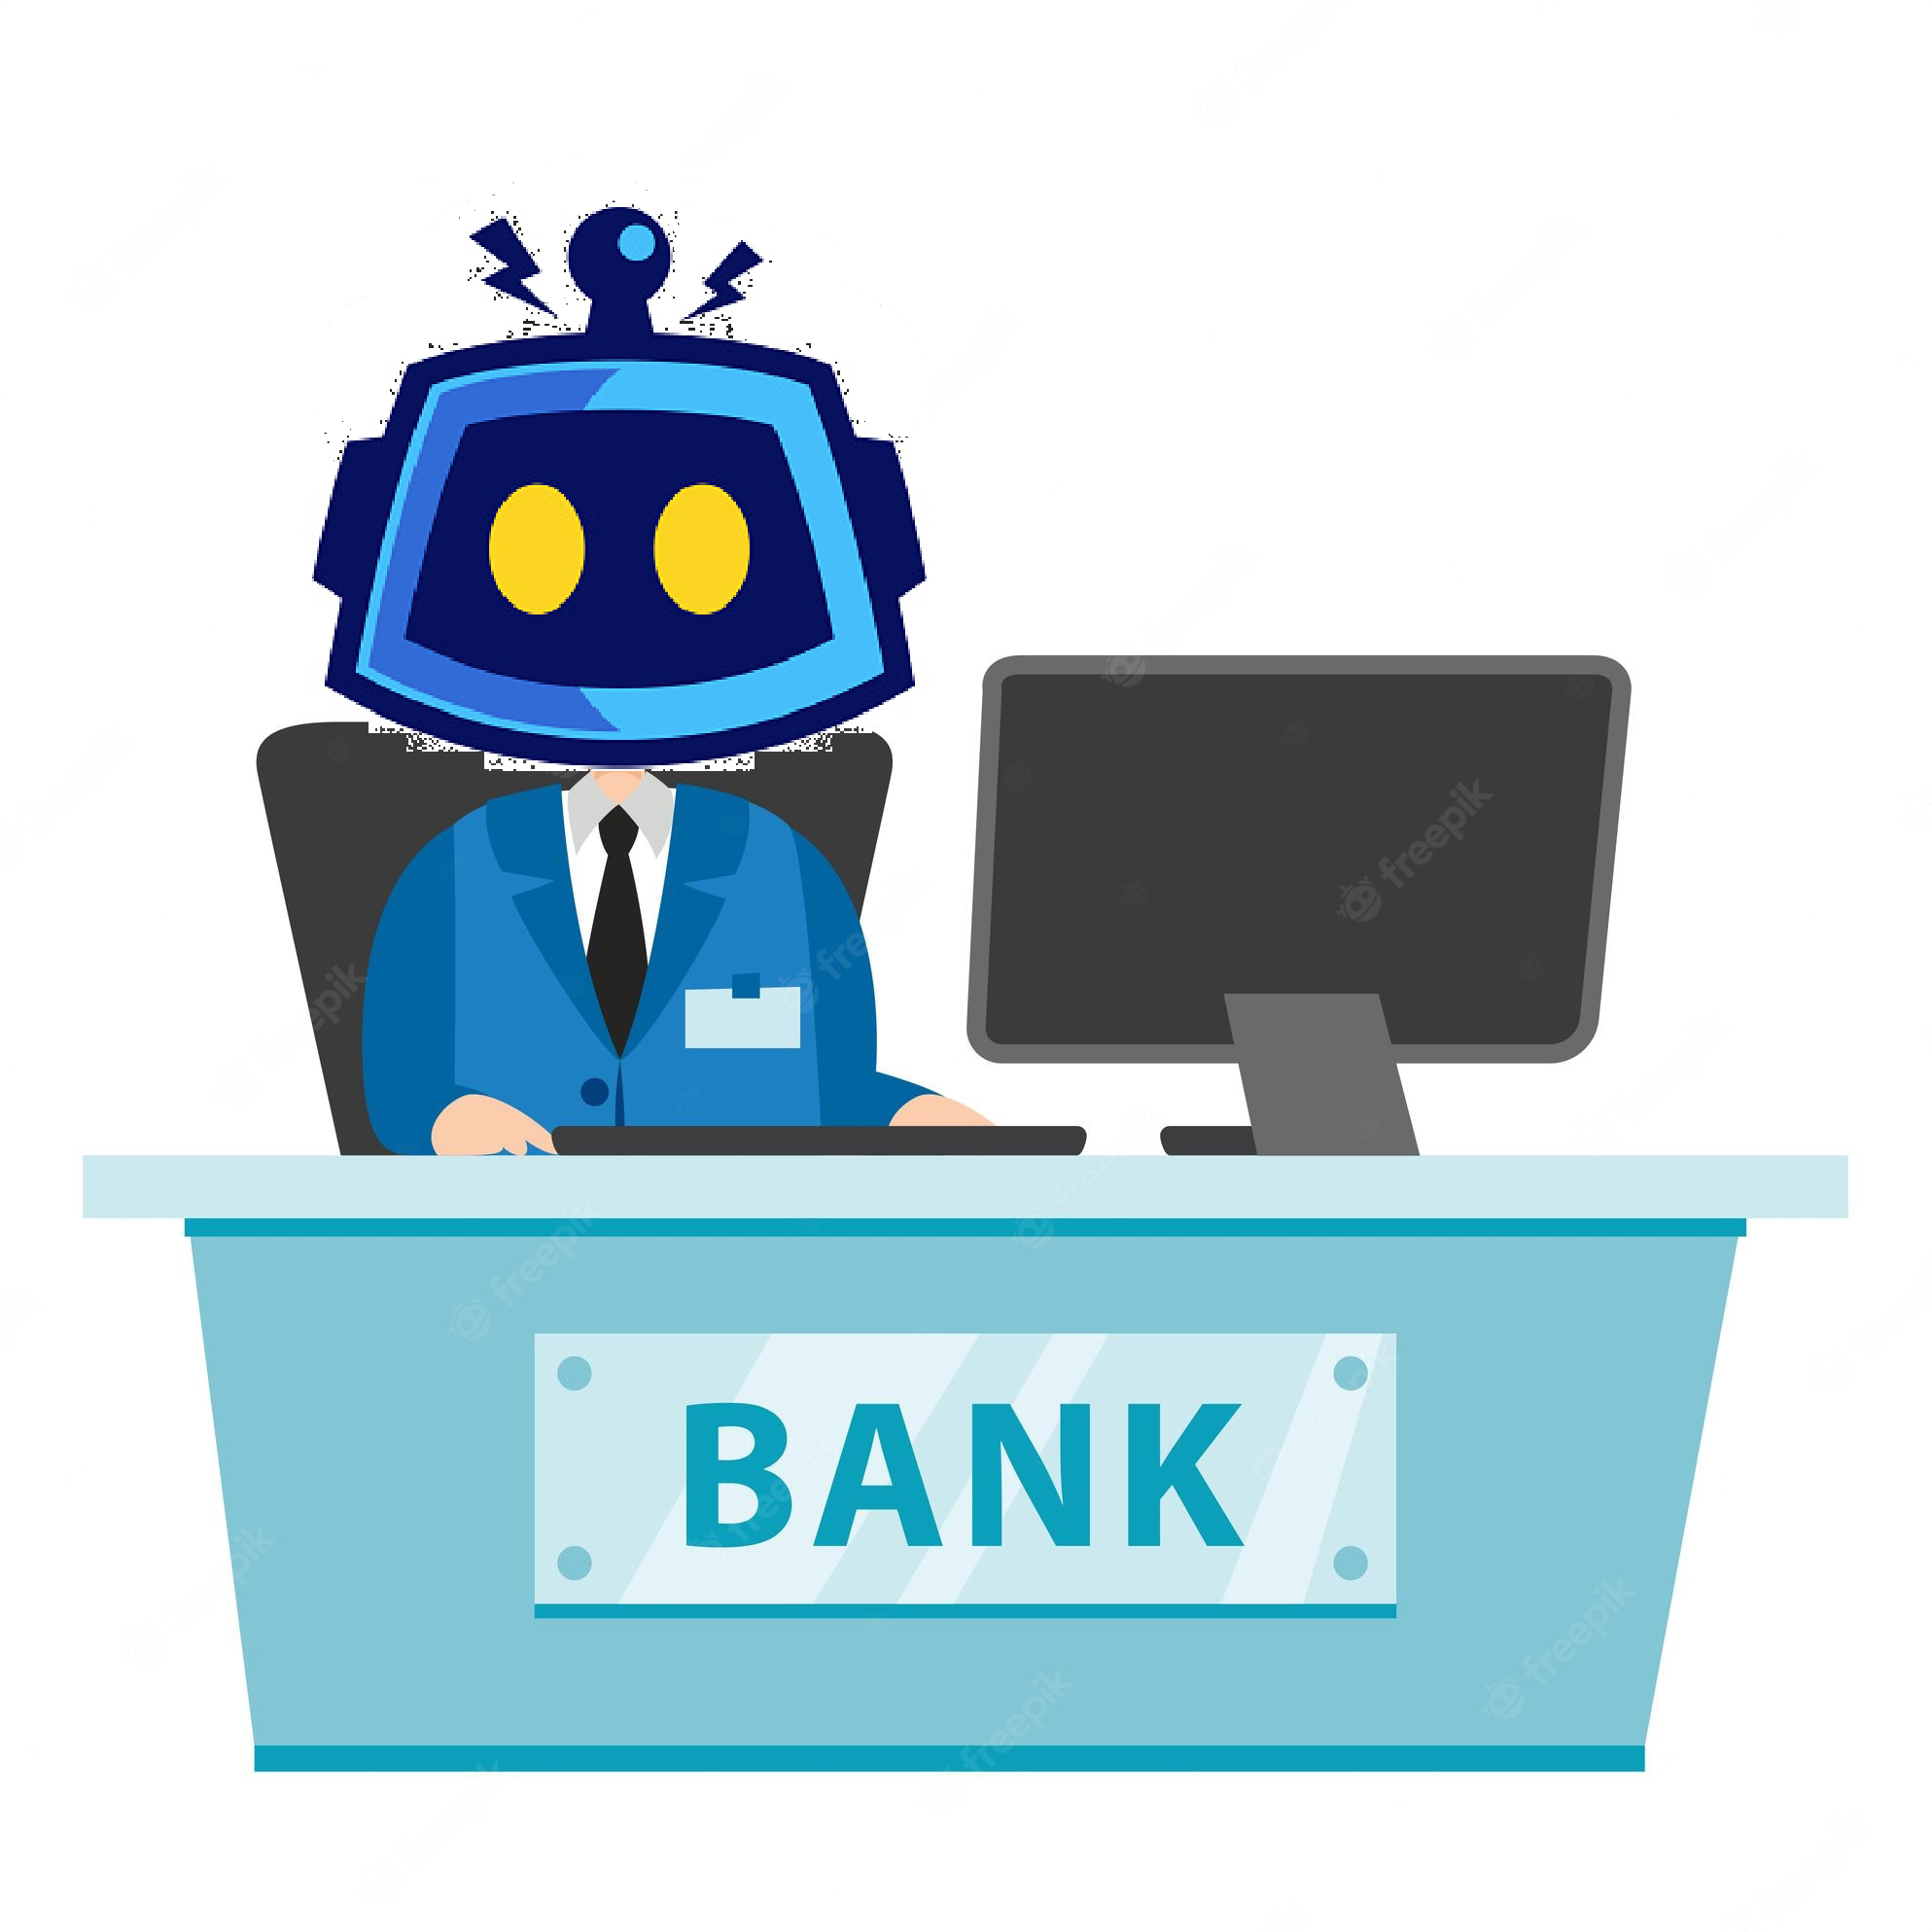
\includegraphics[width=0.2\textwidth]{pics/bankerbot.png}
\end{center}
\bi
\m Governments and courts are \ul{discretionary by default}
\bi
\m Cons: costly, takes time, errors, corruption\ldots
\m Pros: ``rule of reason", better handling of edge cases
\ei \pause
\m Blockchains are \ul{nondiscretionary by default}
\bi
\m Pros: low-cost, ``instant'' outcomes
\m Cons: cannot apply ``rule of reason", unforeseen cases can be handled badly, and hard to reverse!
\ei
\ei

\vspace{3ex}
\small
See ALZ blog post on \href{https://medium.com/@anthonyleezhang/discretion-c037d4d23c78}{discretion}
\end{frame}


\begin{frame}
\frametitle{The Market For Promises: Project Ideas}

\bi
\m Blockchains and discretion:
\bi
\m How do we build discretion? Token courts? Other clever mechanisms?
\m What applications benefit most from discretion? Insurance? Defi ``kill-switches''? Web3 gaming?
\ei
\m The real world asset (RWA) problem:
\bi
\m How do we ``glue'' RWAs to the blockchain? (\href{https://twitter.com/jackchong_jc/status/1574745695654797312}{Many} firms working on)
\m An \ul{oracle} is third party system trusted to tell blockchains what has happened in the real world (\href{https://chain.link/}{Chainlink} clear market leader, \href{https://pyth.network/}{Pyth} a competitor)
\ei
\m The boundaries of the market:
\bi
\m What are forms of rule-based social organization, not served well by the traditional promise enforcement mechanisms, that blockchains could do a better job for?
\m Build a product for these people!
\ei
\ei

\end{frame}

\section{Smart Contracts, Cont.}

\begin{frame}{Explore Uniswap}

\vfill 
\begin{center}
\href{https://app.uniswap.org/explore/pools}{https://app.uniswap.org/explore/pools}
\end{center}

\vfill 
    
\end{frame}


\begin{frame}{Constant Product Automated Market Making}

\textbf{Liquidity Providers} deposit $X$ units of Token $A$ and $Y$ units of Token $B$. They earn fees when the pool is used. 

\begin{center}
    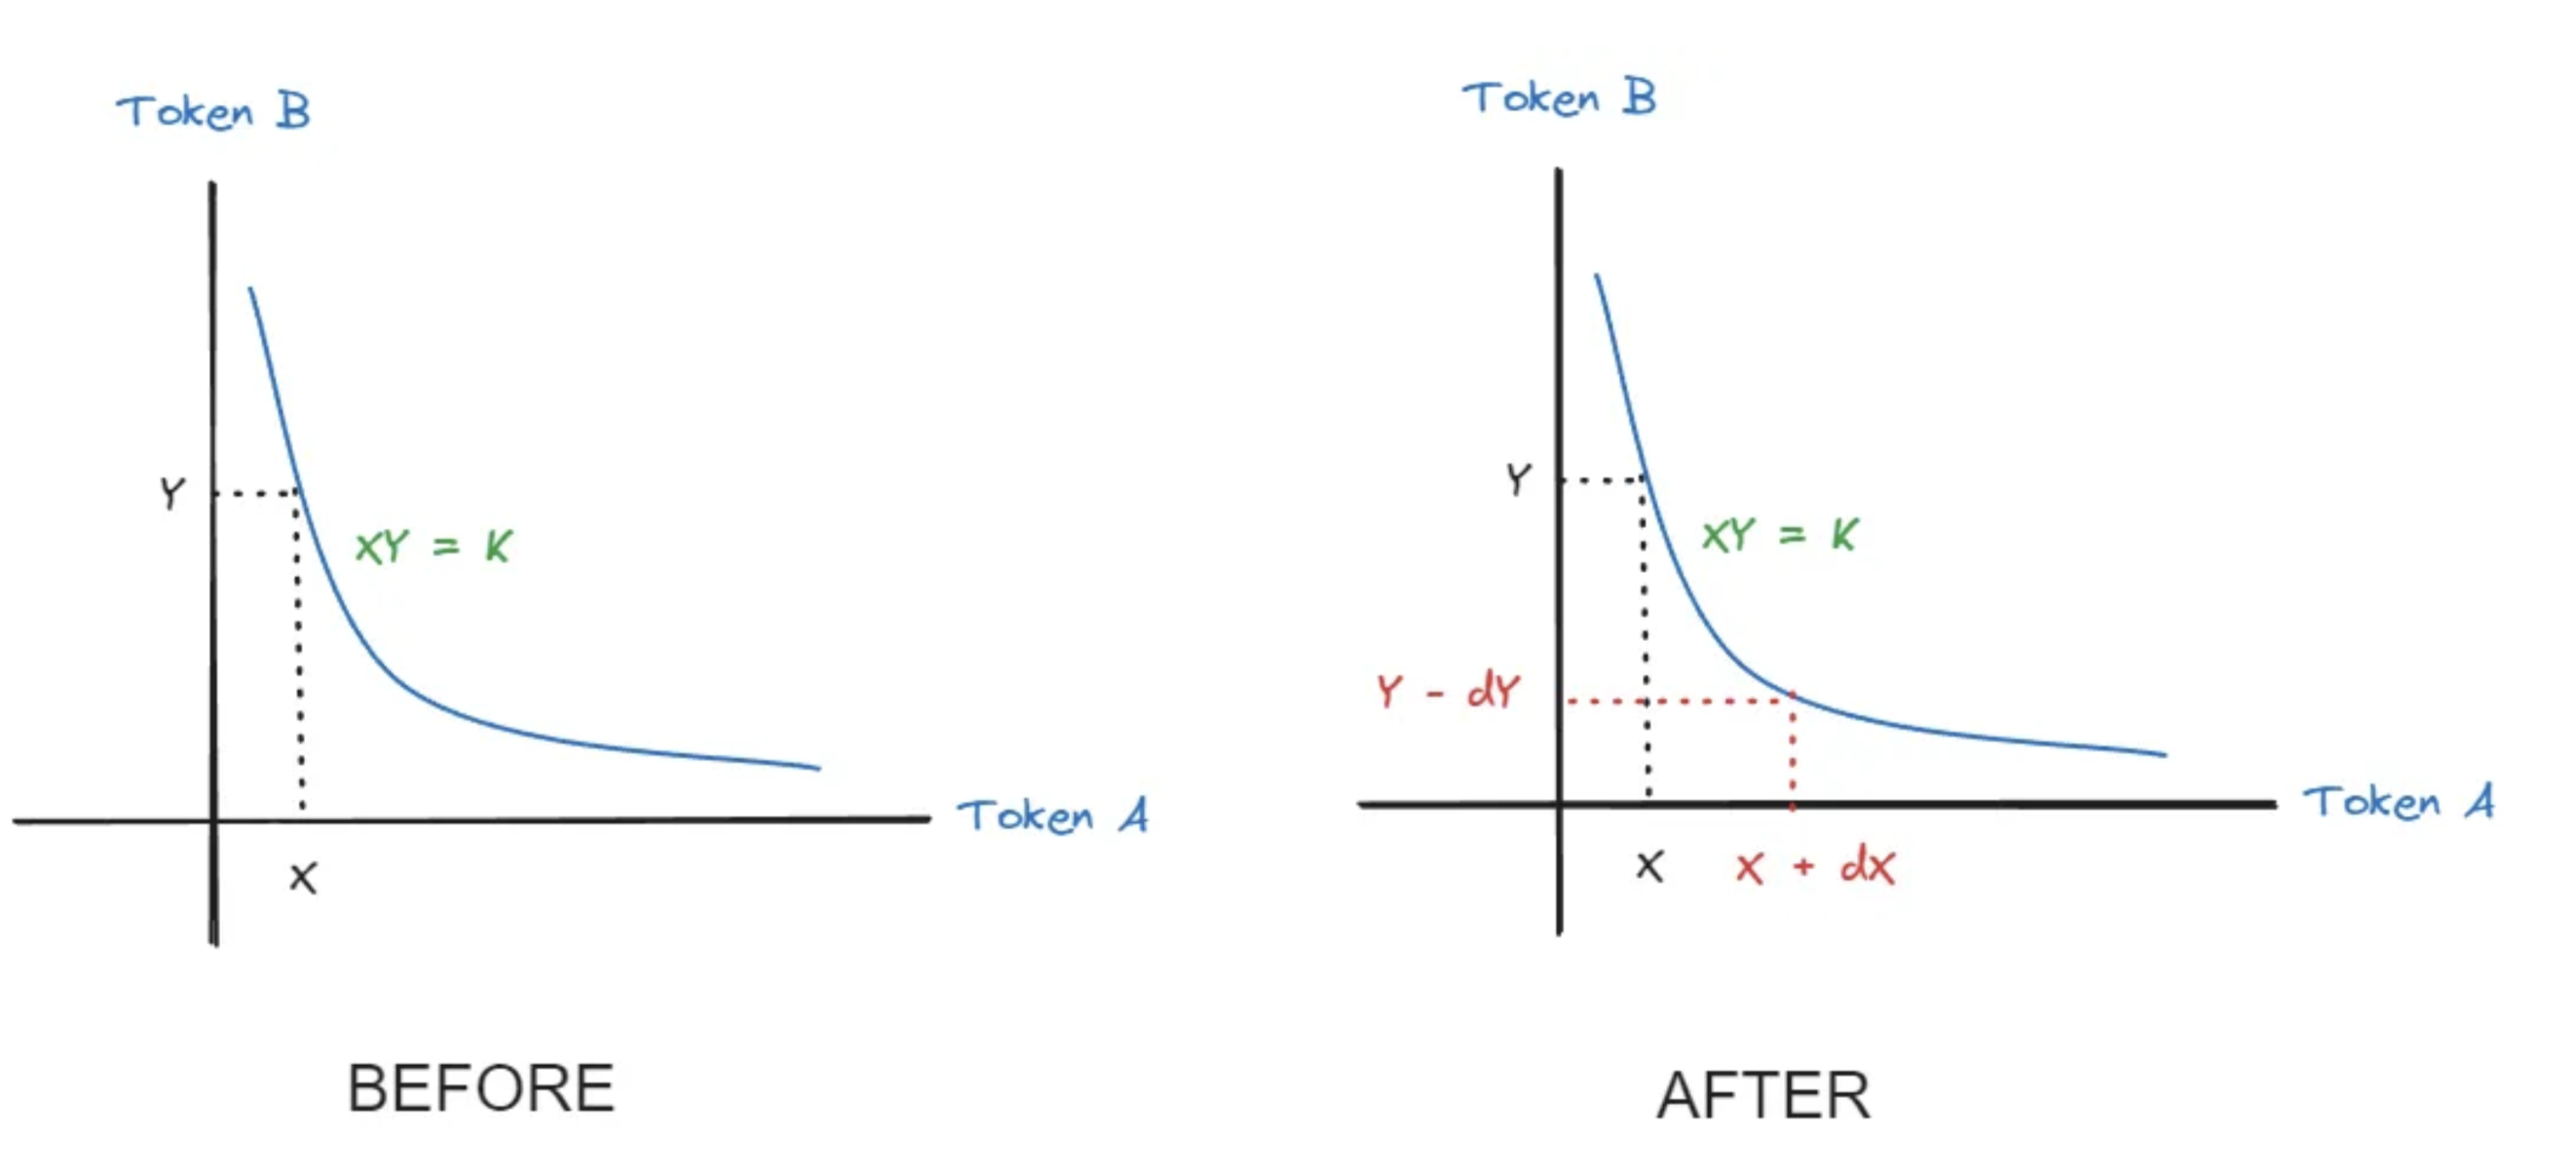
\includegraphics[width = 0.8\textwidth]{Screenshot 2025-02-10 at 5.26.47 PM.png}
\end{center}

Before and after each transaction (a swap or a liquidity injection), the \textbf{constant product rule} $XY = K$ must hold. {\tiny Image Credit: Pari Tomar}

    
\end{frame}


\begin{frame}{Constant Product Rule Math}

\textbf{Q}: Let $X$ and $Y$ be the number of type-x and type-y tokens. When I trade $dx$ type-x tokens, how many type-y tokens will I receive (what is $dy$)? \\ \pause 

The equation 
$$X \cdot Y = K$$
becomes 
$$(X+dx) \cdot (Y-dy) = K$$
\\ \pause 
Substitute $K=X\cdot Y$ and use algebra to isolate $dy$: 

$$dy = \frac{Y\cdot dx}{X+dx}$$
    
\end{frame}

\begin{frame}{Constant Product Rule Math}

\textbf{Q}: When you increase $dx$, does the price move \emph{in your favor} or \emph{against you}?  \\ \pause 

\textbf{A}: Look at the equation and ask what happens when you \textbf{double $dx$}: \pause  the numerator doubles, but the denominator increases as well -- so $dy$ \textbf{less than doubles} -- the price moves \emph{against you}. \\ \pause 

\textbf{Q}: When the liquidity of the pool increases (higher $K$), does this effect (the price moves against you) get stronger or weaker? \\ \pause 

\textbf{A}: Let $X$ and $Y$ be extremely large relative to $dx$ and $dy$. Now, $X+dx \approx X$. In this case, $dx$ and $dy$ are \emph{approximately linear} -- the price movement is close to zero. \textbf{More liquidity means that prices move against you less}. 
    
\end{frame}



\subsection{Gas Fees}

\begin{frame}
\frametitle{How do we police the smart contract ecosystem?}

\bi
\m How to ensure: 
\bi
\m Programs don't run for too long, getting stakers stuck?
\m Programs don't use too much storage, running stakers out of ``hard drive'' space?
\ei \pause
\m Basic idea: \ul{charge people for resources they use}
\m Next, we'll talk about \ul{gas}
\m $10^{-18}$ ETH is called one \textbf{Wei} (for \href{https://en.wikipedia.org/wiki/Wei_Dai}{Wei Dai})
\m $10^{-9}$ ETH is called one \textbf{Gwei} (``Giga-Wei'') 
\ei

\end{frame}

\subsection{Gas}

\begin{frame}
\frametitle{Compiled Code}

\centering
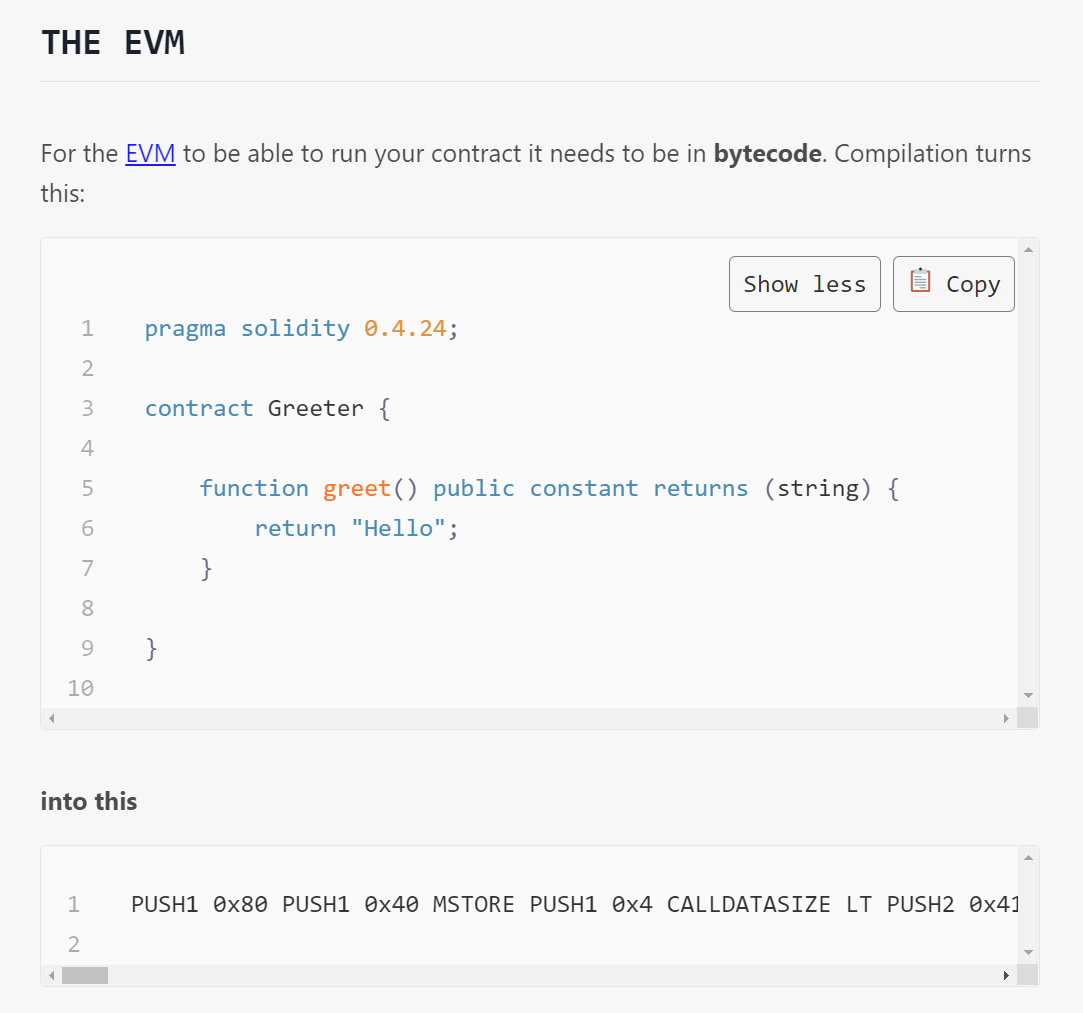
\includegraphics[width=.7\textwidth]{pics/bytecode.png}

\end{frame}


\begin{frame}
\frametitle{Pricing Scarce Computation Resources}

\bi
\m When you run smart contract code, every ETH staker has to run it!
\m When you edit smart contract data, every ETH staker has to store it! \pause
\m Core idea: users pay for the computation + storage resources they use, using ETH
\m ``Computational resources'' used by a function call measured in units of ``gas'' \pause
\m Often unclear how much gas a transaction will take\ldots (``halting problem'')
%\m Tx's specify ``gas limit'': once exceeded, TX fails (but still recorded on the chain!)
%\m Tx's specify ``gas price'' per unit gas, paid to stakers: stakers incentivized to include tx's with highest gas price
\ei

\end{frame}


\begin{frame}{The Halting Problem}

Consider an algorithm (a set of instructions for a computer) $g$. \\ \pause 
Can you define a function $\mathrm{halts(g)}$ which returns $\mathrm{TRUE}$ if the program halts and $\mathrm{FALSE}$ if it will run forever? \\ \vfill 
E.g., if $g$ is \\
$\textrm{while(1==1)\{}$ \\
$\textrm{print(``Another Overtime in the Georgia-Tech Game!'')}\}$ \pause \\ \vfill 

Then $\mathrm{halts}(g)=\mathrm{FALSE}$ -- $g$ does not halt. \pause \\

\href{https://en.wikipedia.org/wiki/Alonzo_Church}{Church (1936)}: No - $\mathbf{halts}(g)$ cannot exist. \pause \vfill 
The shortest possible proof: suppose such a function $\mathrm{halts}(g)$ exists. Then let $g$ be: \pause 
\begin{center}
    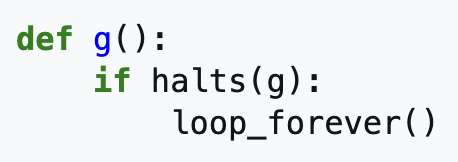
\includegraphics[width = 0.5\textwidth]{Screenshot 2025-02-04 at 6.19.06 PM.png}
\end{center}

    
\end{frame}

\begin{frame}{Unlike BTC, ETH has native gas fees}

``In Bitcoin, there are no mandatory transaction fees. Transactions can optionally include fees which are paid to miners, and it is up to the miners to decide what fees they are willing to accept. In Bitcoin, such a mechanism is already imperfect\ldots In Ethereum, because of its Turing-completeness, a purely voluntary fee system would be catastrophic. Instead, Ethereum will have a system of mandatory fees, including a transaction fee and six fees for contract computations.'' \\

-Ethereum Whitepaper, Vitalik Buterin (2014)
    
\end{frame}


\begin{frame}
\frametitle{Gas Tables}

\begin{center}
\includegraphics<1>[width=.7\textwidth]{pics/bytecode.png}
\includegraphics<2>[width=.8\textwidth]{pics/gastable.png}
\end{center}

\footnotesize
\vspace{2ex}
\href{https://ethereum.org/en/developers/docs/evm/opcodes/}{Source}

\end{frame}

\begin{frame}{Ethereum Virtual Machine Native Gas Costs}

\vfill
\begin{center}
    \href{https://www.evm.codes/}{evm.codes}
\end{center}
\vfill
    
\end{frame}

\begin{frame}
\frametitle{Gas Fees and Smart Contracts}
Meet BankBot (``BB''), a friendly hypothetical smart contract 
\begin{center}
\includegraphics<1>[width=0.2\textwidth]{pics/bankerbot.png}
\includegraphics<2->[width=0.4\textwidth]{pics/bankerbotbill.png}
\end{center} \pause 

\bi
\m BB's actions may cost ETH stakers compute + storage. But BB is a bot!
\m BB only does things when human wallets ask it to\ldots \pause
\m {\ldots}So BB only turns on if you pay for gas \emph{up front}
%\m Human using BB has to pay for computation + data BB uses
\ei

\end{frame}

\begin{frame}
\frametitle{Gas Prices Over Time}

\begin{center}
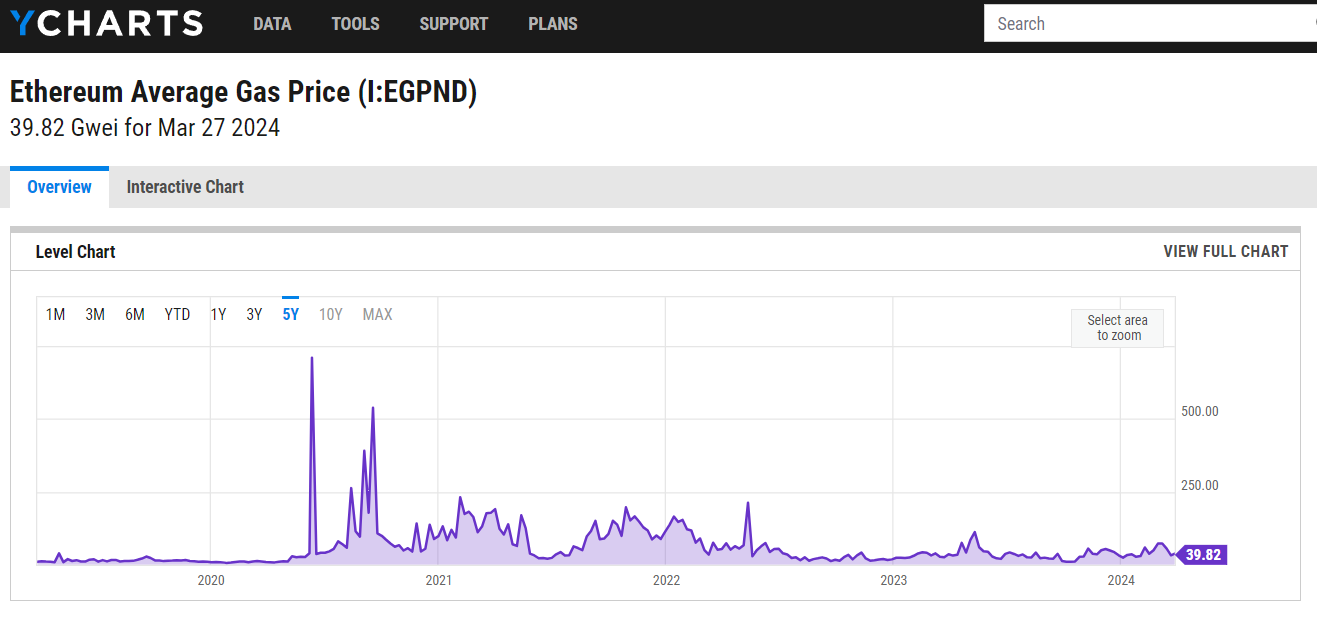
\includegraphics[width=\textwidth]{pics/gaspricechart_2024.png}
\end{center}

\smallskip

\href{https://ycharts.com/indicators/ethereum_average_gas_price}{Source}

\end{frame}

\begin{frame}
\frametitle{Gas Prices and Transaction Demand}

\begin{center}
\includegraphics<1>[width=\textwidth]{pics/otherside1.png}
\includegraphics<2>[width=0.6\textwidth]{pics/otherside2.png}
\includegraphics<3>[width=\textwidth]{pics/otherside3.png}
\end{center}

\end{frame}


\begin{frame}
\frametitle{Capacity of Ethereum}

\bi
\m Ethereum currently processes around \href{https://www.coinbase.com/blog/scaling-ethereum-crypto-for-a-billion-users}{15 transactions per second}
\m This is pretty bad! Visa is \href{https://crypto.com/university/blockchain-scalability}{24,000 tps}!
\bi
\m Every ETH staker has to run every transaction, and keep a copy of all data!
\ei
\m Decentralization very expensive, in terms of computational efficiency!
\m Proof-of-stake doesn't help throughput
\bi 
\m \ul{Rollups} do, which we will cover 
\ei 
\ei

\end{frame}

\begin{frame}
\frametitle{Gas Fees: Summary}

\bi
\m You have to pay to do stuff (sends, smart contracts, etc.) on Ethereum
\m The more computation/storage you use, the more you pay
\m Price depends on overall level of transaction demand
\bi
\m When network is ``congested'' and everyone wants to transact, gas prices high
\ei
\m Next subject: the Ethereum \textbf{user interface}
\ei

\end{frame}

\subsection{User Interface}

\begin{frame}
\frametitle{User Interface}

\bi
\m Like Bitcoin, interact with ETH through wallet software, which helps you manage private keys, sign transactions, etc. 
\m By far most popular ETH wallet software is \href{https://metamask.io/}{Metamask}
\m Metamask is set up as a browser extension
\m \textbf{Warning:} there are many scammers pretending to be Metamask customer support! Just try posting "metamask" on Twitter\ldots
\ei

\vspace{3ex}
\footnotesize

\end{frame}

\begin{frame}
\frametitle{Metamask}

\centering
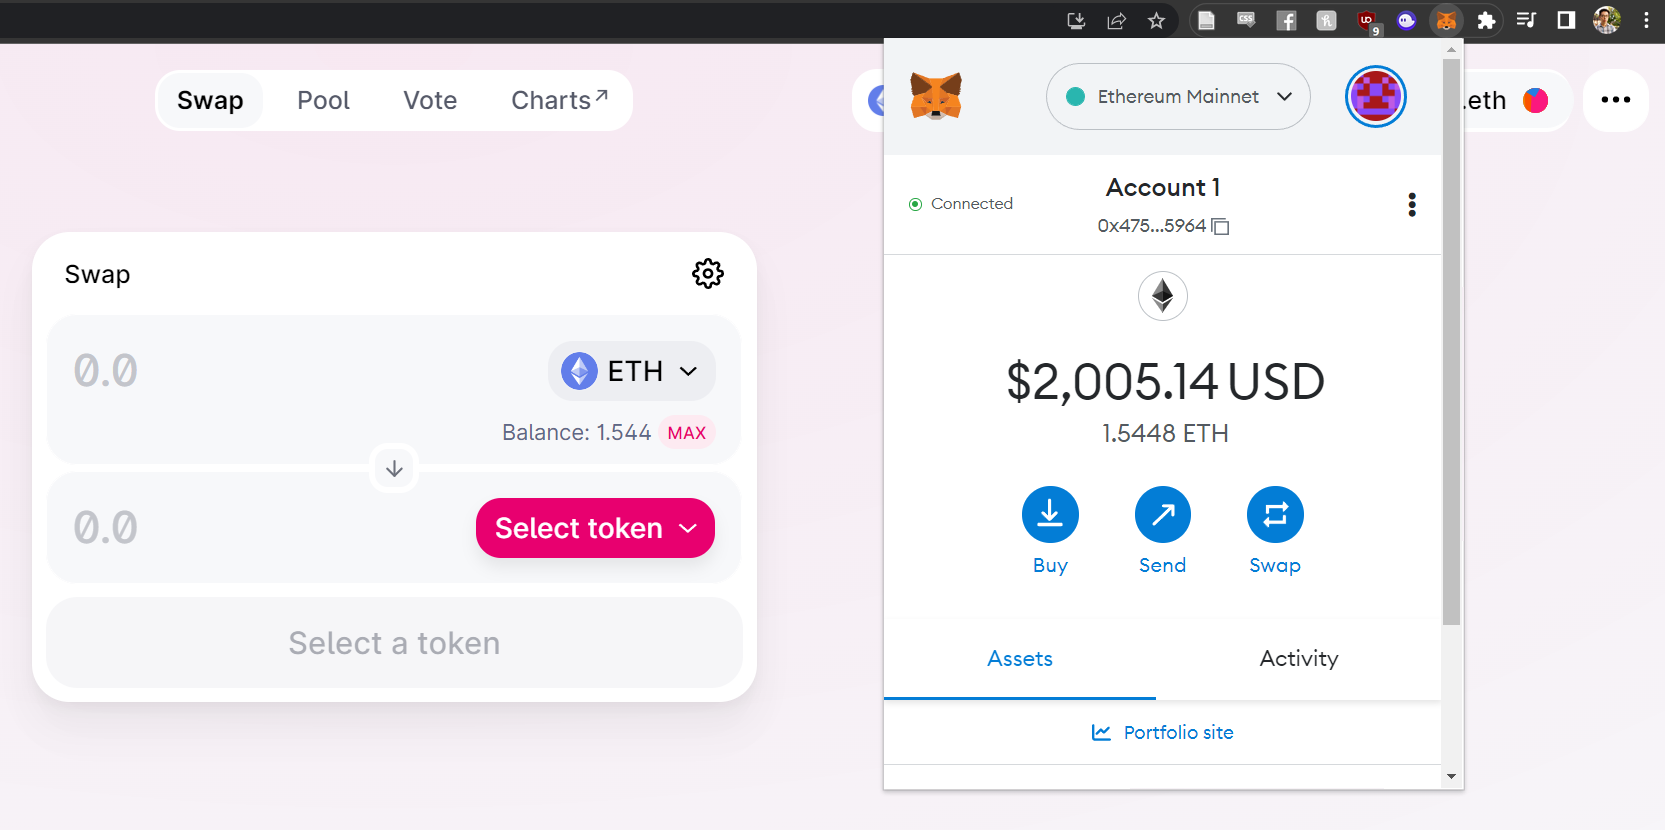
\includegraphics[width=\textwidth]{pics/metamask.png}

\end{frame}

\begin{frame}
\frametitle{Metamask: Private Keys}

\centering
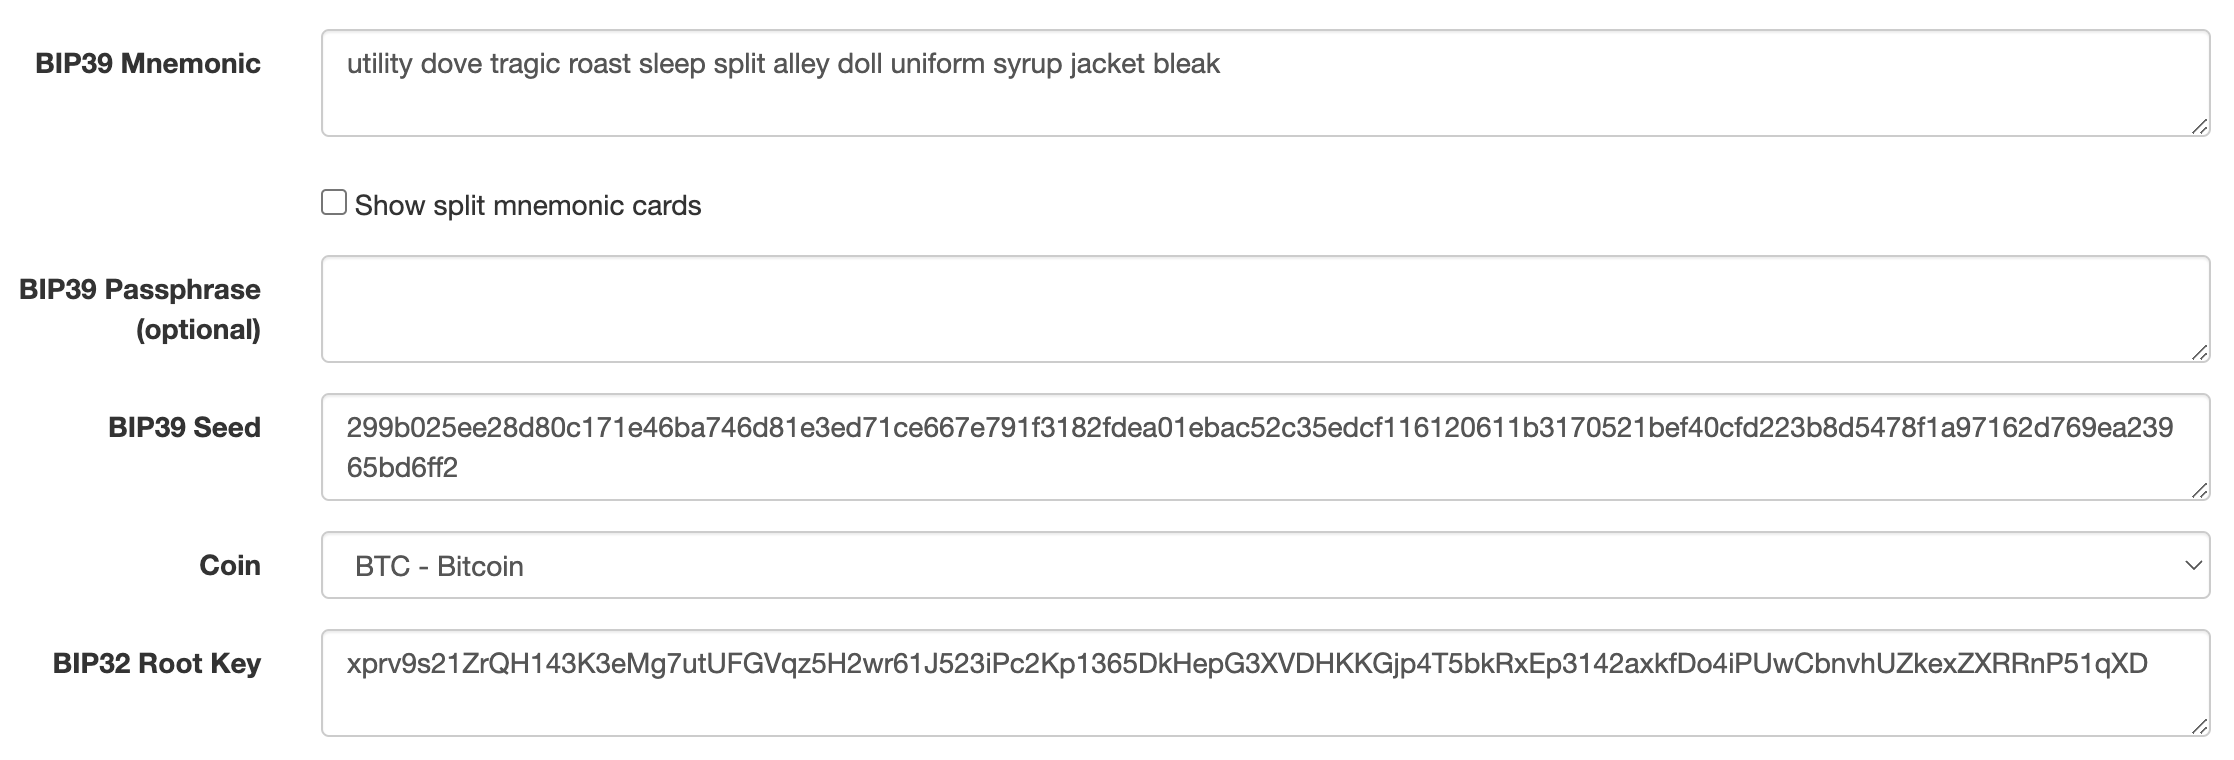
\includegraphics[width=\textwidth]{pics/privatekey.png}

\end{frame}

\begin{frame}
\frametitle{Rule Number 1 of Blockchain Security}

\pause

Never, \pause

\large Never, \pause

\Large Never, \pause

\huge Never, \pause

\Huge Never give out your seed phrase! \pause 

\Huge EVEN IF THEY SAY THEY LOVE YOU

\end{frame}

\begin{frame}
\frametitle{Shamir's Secret Sharing Scheme}
\pause

\footnotesize
See \href{https://blog.trezor.io/https-blog-trezor-io-dev-corner-shamir-backup-guide-5f9957ff1008}{here}
\end{frame}

\begin{frame}
\frametitle{Hardware Wallets}

\bi
\m For better security, use a \ul{hardware wallet}
\m Popular brands include \href{https://trezor.io/}{Trezor} and \href{https://www.ledger.com/}{Ledger}
\bi
\m Common sense: don't buy used! Closed-box from a reputable merchant, and if you're paranoid, reset firmware before using
\ei
\m \ul{If you give away your seed phrase you still lose!} \pause
\m Moral of story: be careful with your crypto!
\ei

\end{frame}


\begin{frame}
\frametitle{Uniswap Example}

\centering
\includegraphics<1>[width=0.8\textwidth]{pics/uni1.png}
\includegraphics<2>[width=0.8\textwidth]{pics/uni2.png}
\includegraphics<3>[width=0.8\textwidth]{pics/uni3.png}

\end{frame}



\begin{frame}
\frametitle{Native Composability}

\bi
\m Web3 (DeFi) gives us \ul{native composability}
\m In web2, app functions and data are \ul{closed by default}
\bi
\m FB, Goog, Twitter have internal functions, data\ldots
\m But can't access each other's data + functions, unless they specifically build APIs to do so
\m If Google doesn't want your app to ``plug into'' Google maps, hard for you to do so
\ei \pause
\m In web3, app functions + data are \ul{open by default}!
\bi
\m Very hard for Uniswap to ``stop'' your app from calling Uniswap functions!
\m All data is on chain: everyone can see every app's data!
%\m Will be important for ``vampire attacks'' in tokenomics lecture in a few weeks
\ei \pause
\m Harder to construct ``walled garden ecosystems'', lower barriers to entry + less incumbent advantage
\ei

\vspace{2ex}
\small
See ``Appendix: Composability'' in Saffron Huang's post \href{https://saffron.mirror.xyz/MEz-IkBGe36LdLn2VVA6grv9FWxU2NdQpVubF6T1ZJE}{here}

\end{frame}

\begin{frame}
\frametitle{Project Ideas: User Interfaces, User Experiences}

Still very early -- this stuff is too nerdy for 99\% of humankind!
\bi
\m UI/UX design is not just ``pretty pictures and buttons''!
\m How can UIs be made more understandable and secure?
\bi
\m What data to display? Users shouldn't have to worry about low-level details of mining, blocks\ldots
\m Better contact books? DNS? Nobody wants to work with these: 0xd8dA6BF26964aF9D7eEd9e03E53415D37aA96045
\m Auto, ML-based security/bug checks? ``Big number'' checks? ``Approval windows?''
\m Examples: \href{https://twitter.com/ExponentialDeFi/status/1576921584341700608}{Exponential}, \href{https://twitter.com/0xsequence}{Sequence}, \href{https://twitter.com/zypsycom}{Zypsy}, and \href{https://twitter.com/AnthonyLeeZhang/status/1577107304755134465}{others}
\ei
\m UIs currently very desktop-focused
\bi
\m Mobile-native? See \href{https://solana.com/news/saga-reveal}{Solana phone}
\m What new applications are enabled by mobile-native web3? 
\ei 
\ei

\end{frame}

\begin{frame}{Faster Horses}
\centering
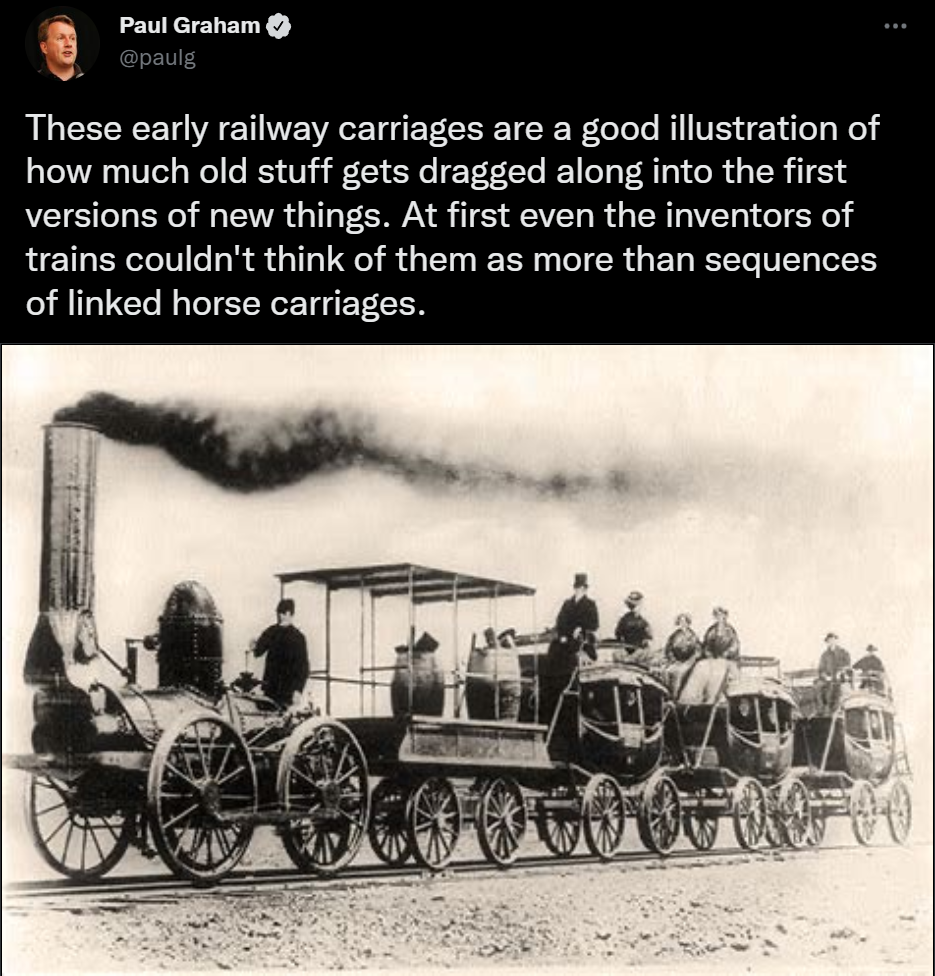
\includegraphics[width=0.7\textwidth]{pics/paulgrahamtweet.png}

\end{frame}

\begin{frame}
\frametitle{Web3 Identity}

\bi
\m What's in a physical wallet? \pause 
\bi
\m Cash, credit cards, and \ul{identity cards}!
\ei
\m An ID card is an item which: 
\bi
\m Proves who you are (student, gym member\ldots) 
\m Gives you certain rights (discounted tickets, gym access\ldots)
\ei
\m ID cards are not transferrable!
\m We can create web3 ID cards through \ul{non-transferable tokens}
\m May 2022 \href{https://papers.ssrn.com/sol3/papers.cfm?abstract_id=4105763}{Weyl-Ohlhaver-Buterin} paper: \ul{soulbound tokens} as the basis of web3 identity
\ei

\end{frame}

\begin{frame}
\frametitle{Project Ideas: SBTs and Web3 Identity}

Identity very young, essentially no apps yet, so a good area for class projects! Many taken from \href{https://papers.ssrn.com/sol3/papers.cfm?abstract_id=4105763}{WOB paper}
\bi
\m What are good SBT use cases?
\bi
\m Diplomas? Employment history?
\m ``Social credit scoring''? Rewards for good deeds?
\m Some examples: \href{https://twitter.com/otterspace_xyz}{Otterspace}, \href{https://twitter.com/discoxyz}{Disco.xyz}, \href{https://lens.xyz/}{Lens}, and \href{https://twitter.com/AnthonyLeeZhang/status/1577104530348859392}{others}
\ei
\m How should SBTs work?
\bi
\m Who gets to bestow SBTs?
\m Who gets to remove SBTs? Privacy? ``Scarlet letter'' SBTs?
\m How do we solve ``walking away from my soul''?
\ei
\m In a world where SBTs are ubiquitous, what functions are enabled that can't exist yet?
\bi
\m SBT-based uncollateralized lending? 
\m SBT-ML and recommendation filtering?
\m SBT-gated social organization? Private clubs? Dating apps?
\ei
\m More broadly, what are some implications of ``native composability'' that the world hasn't realized yet?
\ei

\end{frame}

\subsection{Data}

\begin{frame}
\frametitle{Ethereum Data}

\bi
\m All ETH data is public! However, quite painful to work with
\m Sizable industry has emerged to organize + display ETH data
\ei

\end{frame}

\begin{frame}
\frametitle{Etherscan}

\centering
\includegraphics<1>[width=0.8\textwidth]{pics/etherscan1.png}
\includegraphics<2>[width=0.8\textwidth]{pics/etherscan2.png}

\end{frame}

\begin{frame}
\frametitle{Dune}

\centering
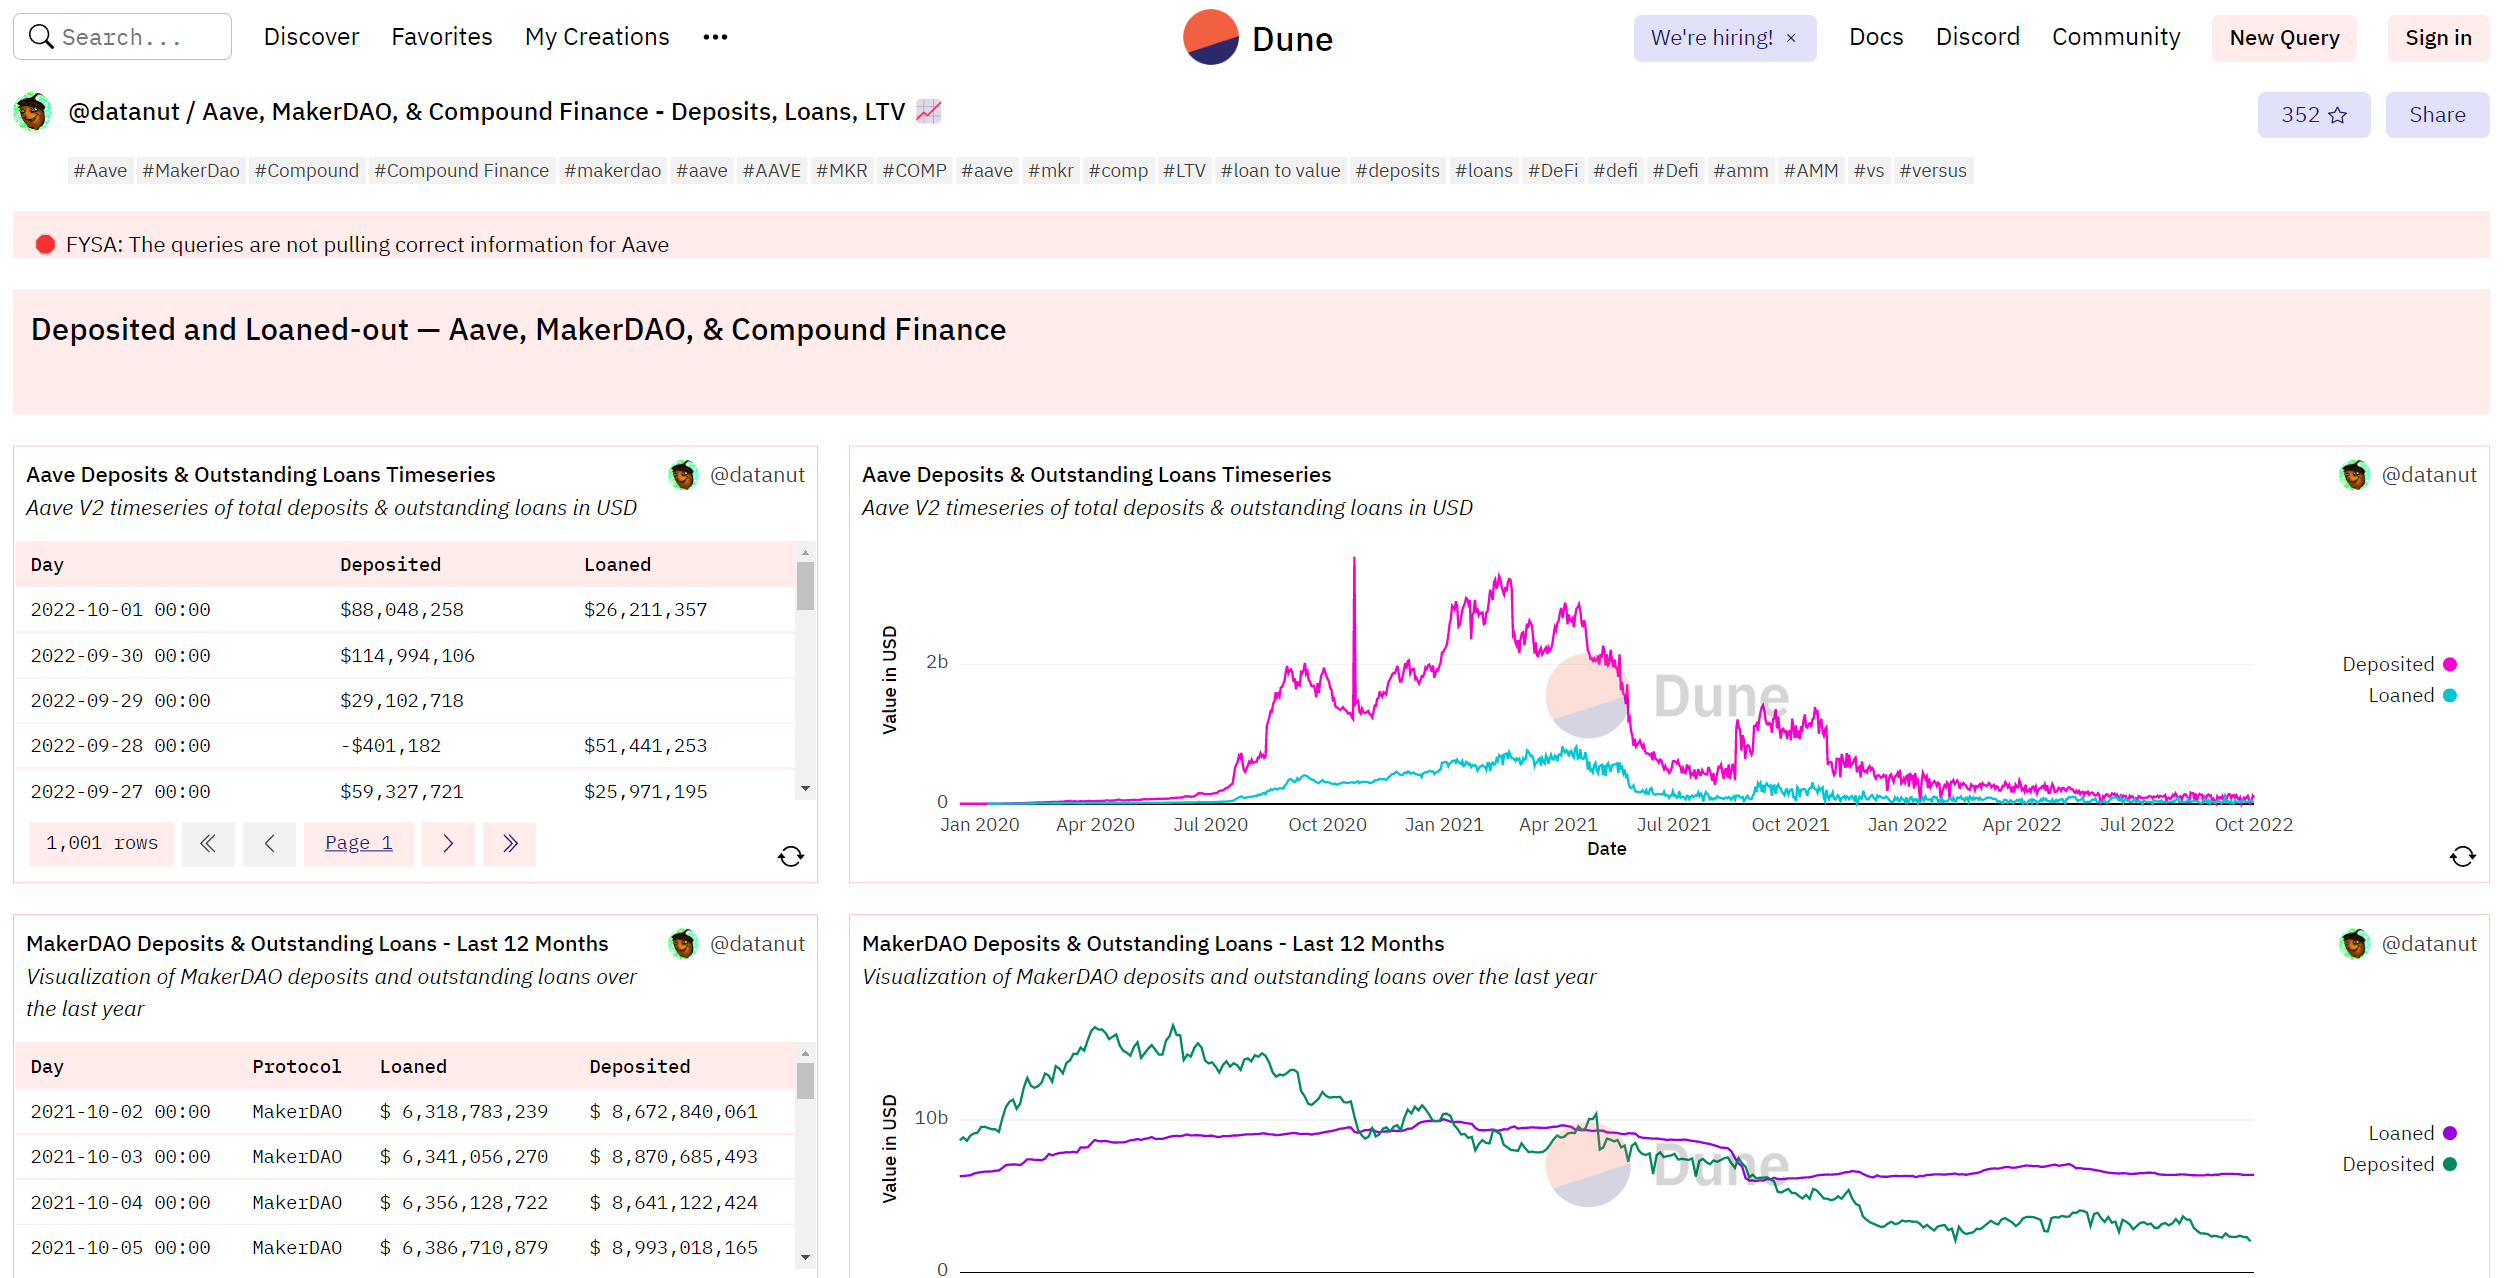
\includegraphics[width=\textwidth]{pics/dune.png}

\end{frame}

\begin{frame}
\frametitle{Nansen}

\centering
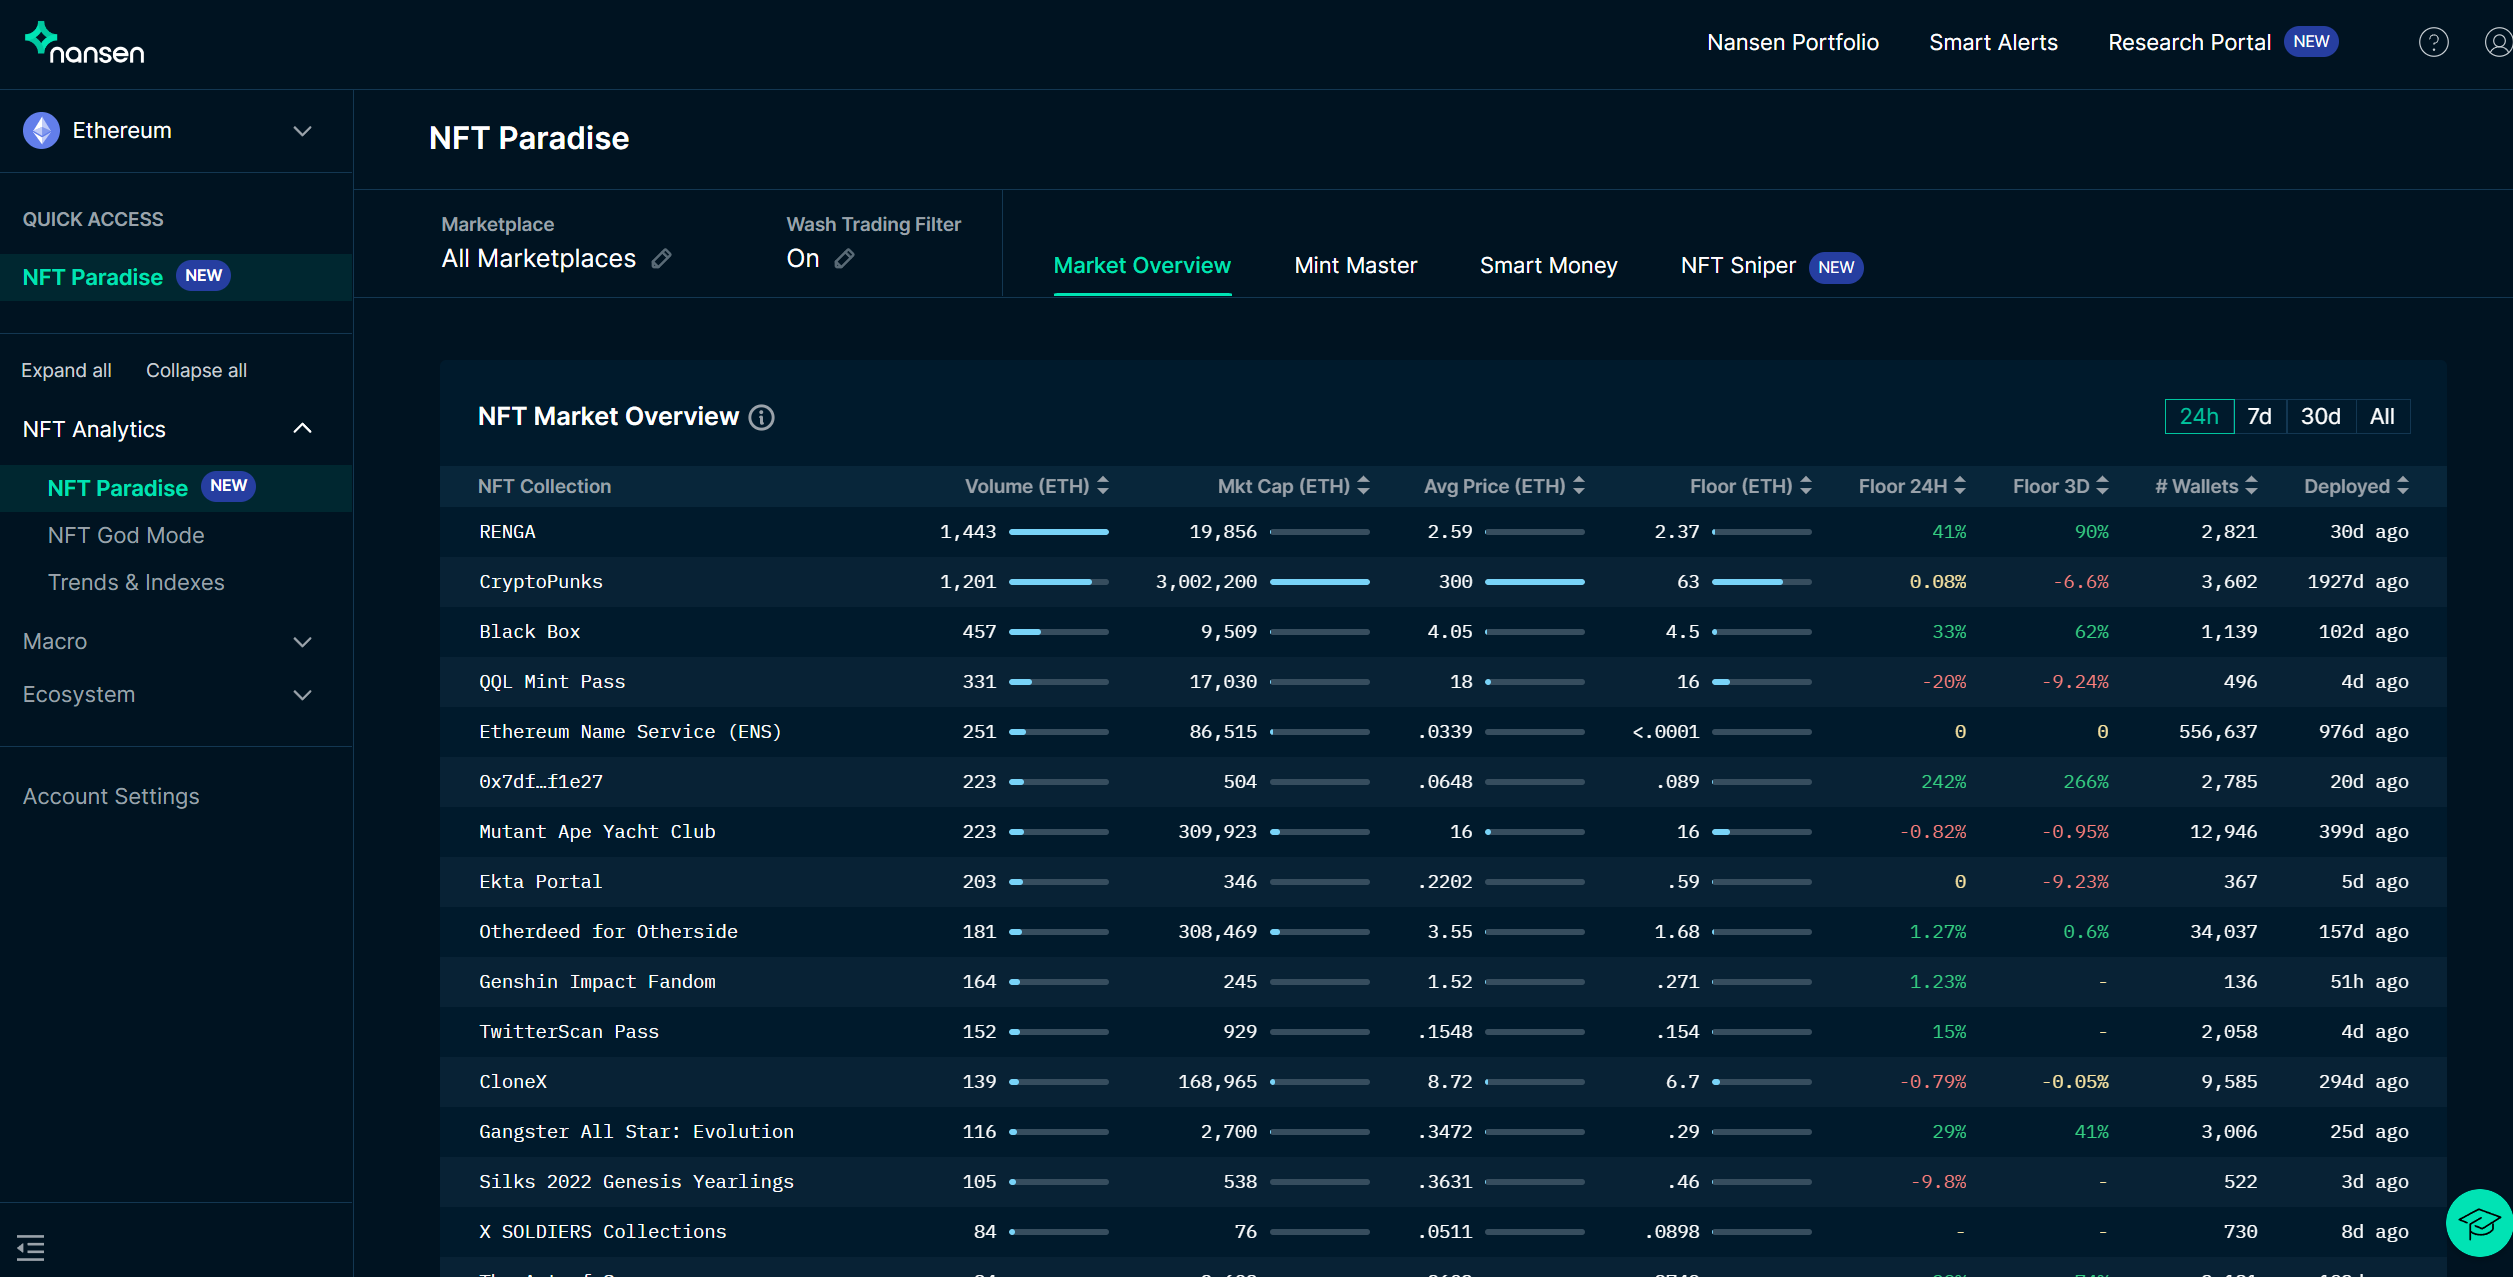
\includegraphics[width=\textwidth]{pics/nansen.png}

\end{frame}

\begin{frame}
\frametitle{Yield Samurai}

\centering
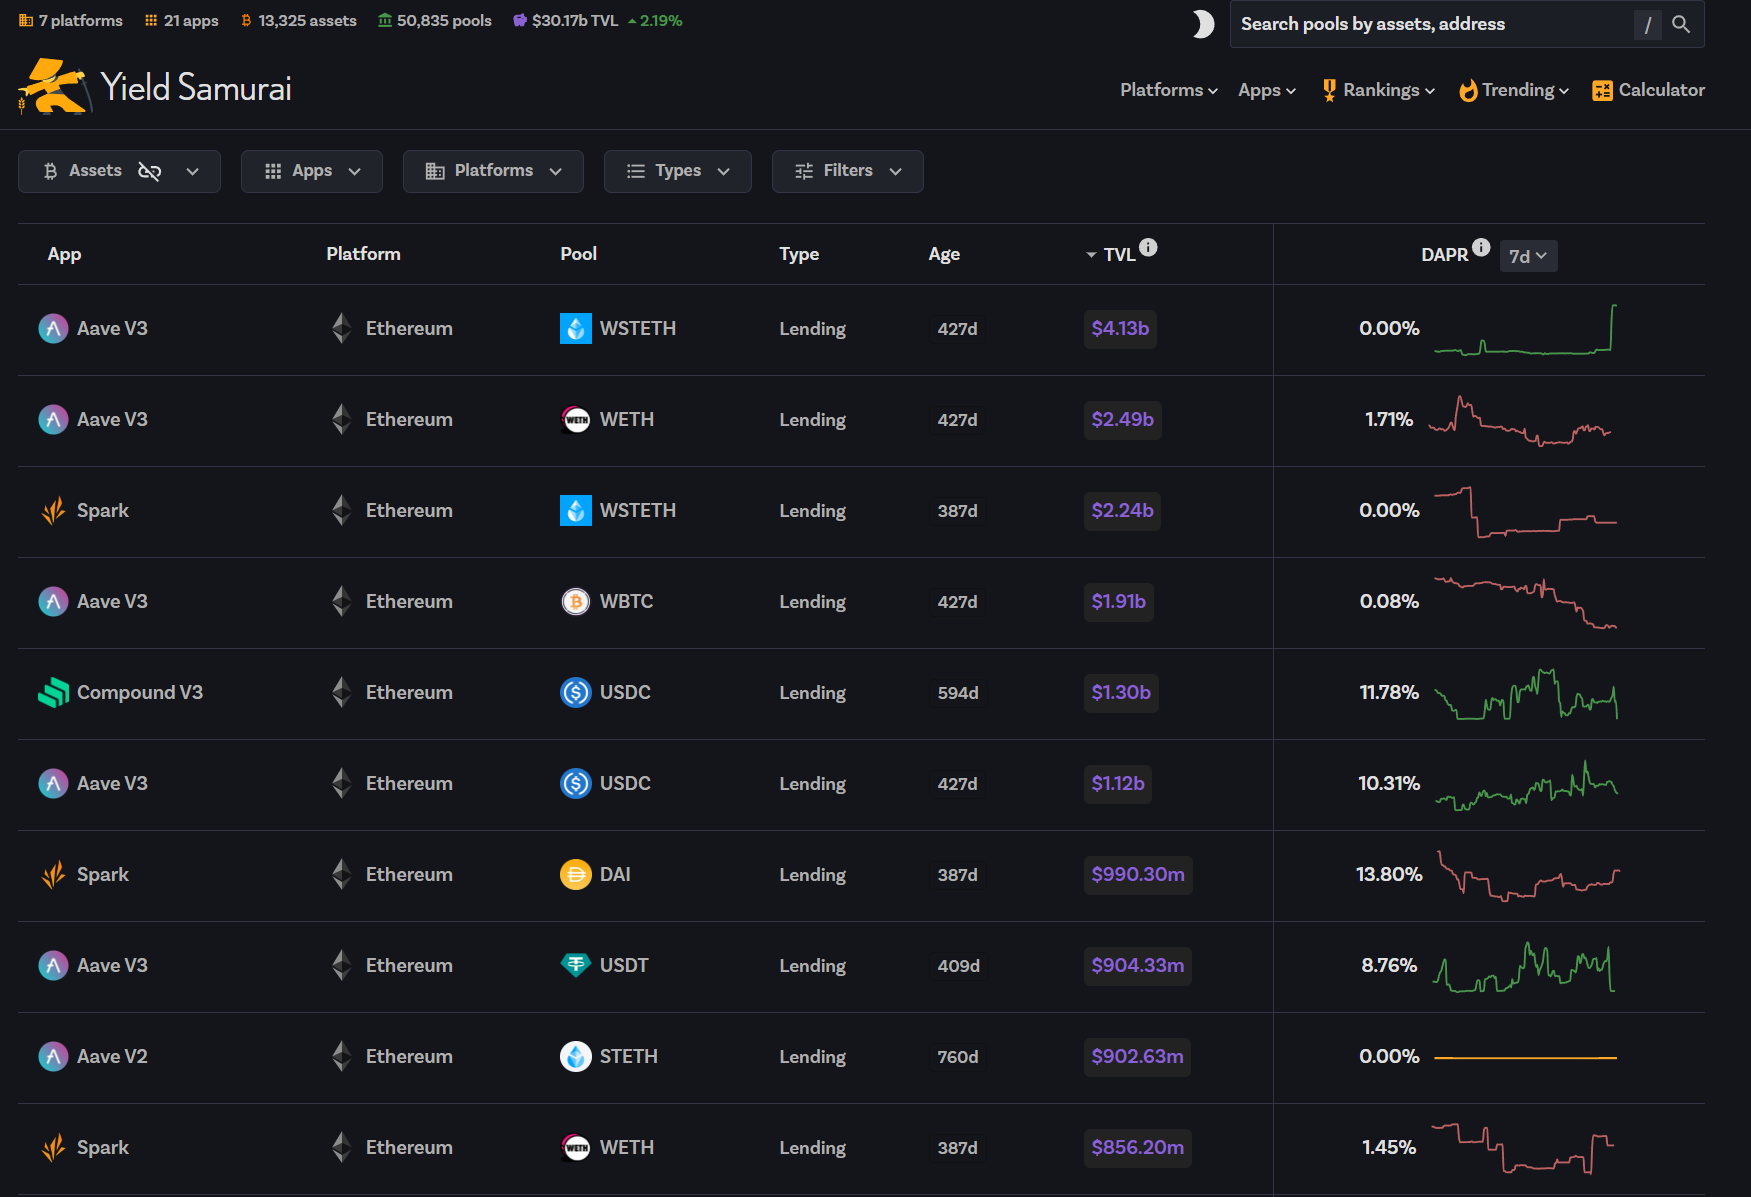
\includegraphics[width=\textwidth]{pics/yieldsamurai.png}

\end{frame}

%\begin{frame}
%\frametitle{Project Ideas: ETH Data Analytics}

%\bi
%\m No data costs: literally everything is public!
%\m Potentially good area for class projects!
%\bi
%\m (Slightly outdated) Recent examples: \href{https://twitter.com/BeckerrJon/status/1577031529464676352}{TransposeData}, \href{https://twitter.com/AnthonyLeeZhang/status/1577111246674927617}{others}
%\ei
%\m Core components:
%\bi
%\m Familiarity with big data pipelines: AWS/Google cloud\ldots
%\m Organize data into useful format: dashboards, ML analytics\ldots
%\m Find a target market: devs, traders\ldots
%\ei
%\ei

%\end{frame}

\subsection{Proof of Stake}

\begin{frame}
\frametitle{Proof of Stake}

\bi
\m Originally, ETH mining proof-of-work, similar to BTC
\m On Sept 15 2022, ETH switched to \ul{proof of stake} -- called \textbf{``The Merge''}
\m Reduced energy consumption by \textbf{over 99\%}! 
\m Users deposit (``stake'') 32 ETH into a special smart contract
\m Stakers randomly selected (prop. to stake) to propose new blocks
\m If a staker is caught trying to do ``bad things'' (e.g. propose 2 inconsistent blocks), they are ``slashed'': staked ETH is removed by smart contract
\m Most newer blockchains (SOL, LUNA, AVAX) use proof-of-stake
\ei

\end{frame}

\begin{frame}
\frametitle{Staking is Very Concentrated!}

\centering
\includegraphics<1>[width=0.8\textwidth]{pics/staking1_2024.png}
\includegraphics<2>[width=\textwidth]{pics/staking2_2024.png}

\vspace{2ex}

\footnotesize
% Source: \href{https://dune.com/hildobby/ETH2-Deposits}{Dune}
Source: \href{https://dune.com/queries/2394100/3927532}{Dune}

\end{frame}

\section{Competition}


\begin{frame}
\frametitle{ETH L2s}

ETH is getting expensive! One set of solutions is \ul{rollups} (also called \ul{L2's}). Idea:
\bi
\m Put our ETH, tokens, etc. in a ``smart contract pot'' (L2 bridge)
\m People do transactions (smart contract, etc.) using funds in the pot, without doing anything on ``main chain"
\m Transactions are periodically batch settled \pause
\m Need to guarantee whatever happens on ``rollup'' is exactly what would happen on ETH main chain! Two methods:
\bi
\m \textbf{Optimistic rollup} (Optimism, Arbitrum, Coinbase Base): Can ``challenge'' L2 transactions, will (essentially) run on L1 if challenged
\m \textbf{ZK-rollup} (zkSync, StarkWare, Polygon): Some math black magic proves validity of transactions
\ei \pause
\m Industry state: 
\bi
\m \$30B locked! ETH market cap is \$408B, stables \textasciitilde\$141B
\m Optimistic rollups somewhat bigger than ZKs
\ei
\ei

\end{frame}

\begin{frame}
\frametitle{ETH L2s}

\centering
\includegraphics<1>[width=0.8\textwidth]{pics/l2beat1.png}
\includegraphics<2>[width=0.8\textwidth]{pics/l2beat2.png}

\smallskip
\footnotesize
Source: \href{https://l2beat.com/scaling/summary}{L2beat}
\end{frame}


	
%\begin{frame}
%\frametitle{Other L1s}

%Proliferation of other ``L1's", doing similar things to Ethereum. Some notable ones:
%\bi
%\m Avalanche, Solana
%\m Luna (now dead)
%\m Cosmos, Polkadot, Polygon
%\m Tron, Binance Smart Chain
%\m Aptos, Sui
%\m Appchains: dydx
%\m Others?
%\ei

%\end{frame}

%\begin{frame}
%\frametitle{Other L1s}

%\bi
%\m ETH still largest by market cap (behind BTC)
%\m Many newer L1's ``faster'' and ``cheaper'' than ETH
%\m L1's highly concentrated in terms of development/funding: often large ``ecosystem funds'' to promote using/building on 
%\m Still few compelling applications on alt-L1's 
%\m ETH remains the market leader among ``utility'' L1's \pause
%\m \textbf{Project ideas}: Proposing a new L1/L2 is a hard engineering problem and one I don't recommend it to most 
%\bi
%\m If you are an engineer and ``built different'', please by all means blow my mind! 
%\ei
%\ei

%\end{frame}

%\subsection{Governance}

%\begin{frame}
%\frametitle{The DAO Incident}

%\bi
%\m In 2016, org called ``The DAO'' raised \$150mil USD of ETH
%\m Hacker exploited a bug and stole \$60mil\ldots \pause
%\m ETH developers proposed a ``hard fork'': roll back Ethereum to before hack happened, and update the code to fix the bug! 
%\m But the ``non-forked'' chain continues to exist, as ``Ethereum Classic''
%\ei

%\end{frame}


%\begin{frame}
%\frametitle{Centralization and Governance}

%\bi
%\m Even a ``decentralized'' chain like ETH, in practice has influential ``central'' parties (developers)
%\m ``Centralized'' chains, who run chain validation themselves, have even more power
%\m Should chain operators have power to unilaterally influence chain outcomes?
%\m U.S. congress is \textbf{utterly asleep at the wheel}
%\ei \pause

%\textbf{Policy questions}
%\bi
%\m What are the roles and obligations of chain operators?
%\m How much discretion should chain operators have to rollback changes?
%\ei

%\end{frame}




\end{document}
